\documentclass[11pt, oneside]{article}   	% use "amsart" instead of "article" for AMSLaTeX format
\usepackage{geometry}                		% See geometry.pdf to learn the layout options. There are lots.
\geometry{letterpaper}                   		% ... or a4paper or a5paper or ... 
%\geometry{landscape}                		% Activate for rotated page geometry
\usepackage[parfill]{parskip}    		% Activate to begin paragraphs with an empty line rather than an indent
\usepackage{graphicx}				% Use pdf, png, jpg, or eps§ with pdflatex; use eps in DVI mode
\usepackage{caption}
\usepackage{subcaption}
\graphicspath{ {Users/hld523/Reports/my-plasma-report/Figures/} }								% TeX will automatically convert eps --> pdf in pdflatex		

\usepackage{amssymb}
\usepackage{amsmath}

%SetFonts

%SetFonts


\title{Plasmaaaaa}
\author{The Author}
%\date{}							% Activate to display a given date or no date
\begin{document}
\maketitle

\section{Abstract}

The highly reactive nature of reactive oxygen and nitrogen species, and their ability to influence a range of biomolecules indicates their potential for use in biomedical applications such as the promotion of wound healing, bacterial inactivation and cancer treatments.
It is therefore of interest to develop a means of producing these radicals for use in therapies and therein lies the potential of low temperature plasmas.
These plasmas operate at temperatures that are not harmful to biological tissues, and are potent producers of a range of reactive oxygen and nitrogen species (RONS).
Presented here is the characterisation of hydroxyl radical ($\cdot$OH) production in a low temperature, atmospheric pressure, radio frequency plasma.
Data presented here show that increasing power and water content increases the density of $\cdot$OH in the plasma, whilst increasing the water content decreases the degree of dissociation, presumably due to the increased energy consumption for excited rotational and vibrational states of the water molecules.
Further to this, the spatial resolution of $\cdot$OH along the 30 mm plasma channel, and it's decay beyond the plasma region was investigated. These data were then compared to a global chemistry model which gave indications of the dominant reaction pathways for the production and consumption of $\cdot$OH.
Further validation of these results are required in the future but take us one step closer in the characterisation of the RF plasma jet which will hopefully help with future tuning of plasma jets to tailor them for specific therapies.

\section{Introduction}

\subsection{Reactive Oxygen and Nitrogen Species in Biology} \label{sec:RONSinBiology}

Reactive oxygen and nitrogen species are highly reactive molecules, which include free radicals and other non-radical species. 
Free radicals, such as hydroxyl and superoxide radicals, are atoms or molecules with a single, unpaired electron in their outer shell \cite{PhamHuy2008}. 
This free electron results in an extremely high propensity to react with molecules nearby. 
In biological settings, these species are capable of attacking proteins, lipids and DNA \cite{PhamHuy2008} which can lead to their deleterious effects such as mutations.
Other highly reactive molecules such as ozone and hydrogen peroxide are not free radicals in that they do not have an unpaired electron in their outer shell, however, they are still strongly reactive and are capable of reacting to produce free radicals \cite{PhamHuy2008}.

In the past, it was thought that these RONS were solely damaging molecules present in the body that led to ageing and age-related diseases.
These thoughts were termed the free radical theory of ageing \cite{Harman1955}. 
However, since then, it has been shown that, whilst RONS do have a large role in many pathologies, such as diabetes, cardiovascular disease and neurodegenerative disorders, amongst many others \cite{Valko2007}, they are also believed to be important molecules involved in normal physiological functioning.
Of particular interest is the role of free radicals in bacterial killing during an immune response.
Certain immune cells, known as phagocytes, whose job it is to engulf and kill invading pathogens, produce free radicals and other reactive species, such as superoxide, hydrogen peroxide and hydroxyl radical, to kill the engulfed pathogen in a process known as the respiratory burst \cite{Janeway2011}
The importance of this process is shown by patients with chronic granulomatous disease who lack the enzyme required for superoxide production. This means their immune cells cannot produce superoxide in the respiratory burst and predisposes the individual to multiple, persistent infections \cite{Janeway2011, Babior2004}.


This ability to kill bacteria, has led to the idea that these reactive species may provide a potential alternative to conventional bactericidal therapies such as antibiotics, the resistance to which is proving to be a huge challenge in the world today. 
By understanding the role of RONS in the normal functioning immune system, it my provide details of how we could manipulate these species for use in biomedical applications such as bacterial killing in chronic or infected wounds.
However, in order to do this, there would need to be a mechanism for producing and administering the RONS in suitable concentrations.
This is an issue due to the short lived, highly reactive natures of the species.
Recently, there has been much research into the development of low temperature atmospheric pressure plasma jets, which are plasma sources operated at temperatures that are low enough to not be damaging to biological samples, such as the skin, and are potent producers of RONS. 
Low temperature plasmas and their production of RONS will be the focus of the rest of this project.


%RADICALS KILL STUFF, THEREFORE, USE PLASMA!!

\subsection{What is plasma?}
Plasma is the fourth state of matter, formed when energy is increased in a gas, causing some of the gas particles to become ionised \cite{Fridman2013PlasmaMedicine}. 
The degree of ionisation of a plasma refers to the proportion of gas molecules that are ionised.
This depends largely on the energy of the system. 
The higher the energy, the greater the degree of ionisation and therefore the higher the density of free electrons (electron density).
The process of ionisation of gases results in free electrons within the plasma region, which gives the plasma it's properties.
Plasmas are said to be quasi-neutral, meaning that whilst they contain many charged particles, overall, there is no charge to the system.

\subsection{Low Temperature Atmospheric Pressure Plasmas} \label{section:LowTempPlasmas}

Plasmas can range from being almost fully ionised, to very weakly ionised.
Highly ionised, very hot plasmas, such as the sun, exist at very high overall temperatures. 
This is due to a state of thermodynamic equilibrium being reached. 
For this to occur, free electrons are accelerated across a potential difference and gain energy which they then impart to other ions and neutrals through collisions.
Although energy transfer between very small electrons and much bigger neutrals and ions is poor, if there is sufficient energy in the system, then all the particles within the plasma will end up 'hot', $T_e \approx T_i \approx T_g$ (where $T_e$ is electron temperature, $T_i$ is ion temperature and $T_g$ is gas temperature).

However, at the other end of the scale are low temperature plasmas. 
These plasmas are only weakly ionised and therefore have low degrees of ionisation and low electron densities.
For these plasmas, thermodynamic equilibrium is never reached due to the poor energy transfer between electrons and bigger ions and neutrals. 
This results in a state where $T_e >> T_i \approx T_g$ and therefore, overall, the temperature of the plasma remains cool at approximately room temperature.
It is this ability to produce plasmas at low temperatures that makes them so exciting in the field of biomedicine and only these types of plasmas will be considered from now on in this report.

Electrons in plasma have a range of energies which forms an electron energy distribution function (EEDF) as shown in figure \ref{fig:EEDF}.

\begin{figure}
	\centering
	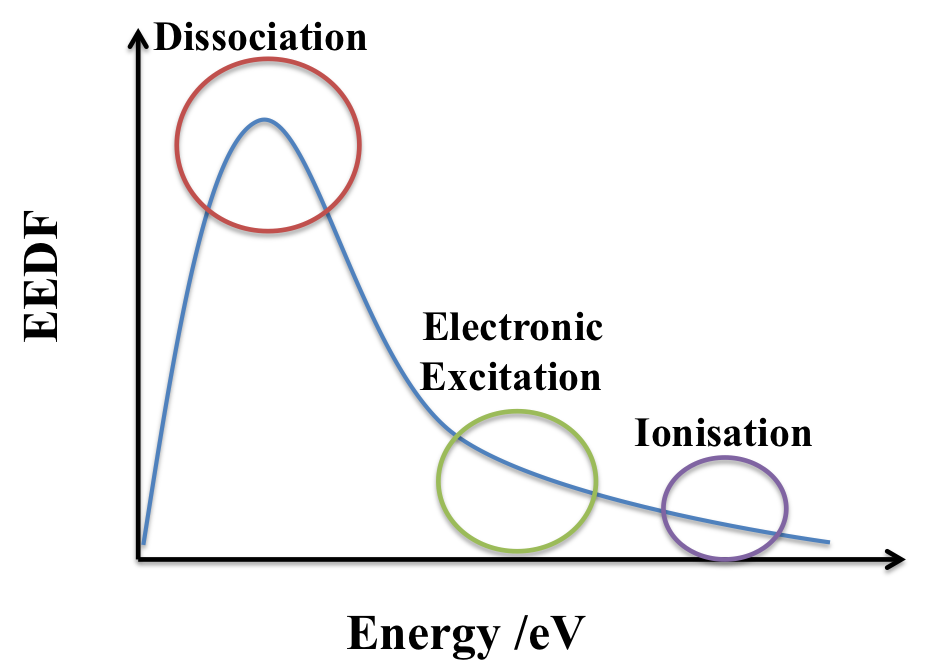
\includegraphics[width=0.7\textwidth]{Figures/EEDF}
	\caption{Diagram showing a typical plasma EEDF curve and the different processes occurring at different electron energies. There are more lower energy electrons than high energy electrons.}
	\label{fig:EEDF}
\end{figure}

The three main processes that electrons mediate are:
\begin{itemize}
\item Dissociation - electron impact causes splitting of molecules. This is the mechanism by which, for example, molecular gases become atomic and how free radicals can be produced (figure \ref{fig:EEDF}, red circle)
\item Electronic excitation - electron impact can excite an atom/molecule by causing one of it's electrons to be promoted to a higher energy orbital if the impacting electron's energy matches the difference in energy between orbitals. Following this, the atom/molecule can relax back to a lower energy level, and in doing so, emits a photon with energy equivalent to the difference between energy levels. This is how the visible light from plasma is emitted (figure \ref{fig:EEDF}, green circle)
\item Ionisation - If the electron energy is sufficient, on collision with another atom or molecule it can cause an electron to be knocked off the particle and result in it's ionisation and a free electron being released. This is the mechanism by free electrons are always being produced in order to sustain the plasma and counteract the loss of electrons due to recombination (figure \ref{fig:EEDF}, purple circle)
\end{itemize}

Electrons in low temperature plasmas have typical mean energies in the range of 0.5 - 5 electron volts (eV), much greater than energies of larger neutrals and ions (0.025 - 0.05 eV), but much less than the energies required for dissociation, electronic excitation and ionisation \cite{Christophorou2012}.
However, a small fraction of the electrons are able to attain energies sufficient to carry out these processes and therefore sustain a plasma.

\subsection{Biomedical Applications of Low Temperature Plasmas}

High temperature plasma has a history of use in the field of biomedicine for uses such as sterilisation and cauterisation, among others.
However, the emerging field of low temperature plasma research is resulting in the development of plasmas which can operate at low, non harmful temperatures, whilst still producing large quantities of RONS capable of influencing many biomolecules such as cell membranes, DNA and other cellular components \cite{Graves2012}.
Herein lies the potential for biomedical applications of low temperature plasmas.
For example, promotion of wound healing, killing of cancer cells and bacterial inactivation may all be possible using plasma treatment.
One plasma device already in use for the promotion of chronic wound healing is PlasmaDerm \cite{BrehmerHD2015}.
Alongside the production of RONS, plasma treatment also involves electric fields and ultraviolet radiation interacting with the surface being treated.
This multimodal nature of plasma treatment could mean that resistance to treatment by it may not occur. 
This would be beneficial in this era of increasing antibiotic resistance.



\subsubsection{The Hydroxyl Radical ($\cdot$OH)} \label{sec:HydroxylRadical}

The types of RONS produced by the plasma depend on the feed gas and the power supplied to the plasma.
For example, a helium feed gas with admixtures of oxygen will yield reactive oxygen species such as ozone, superoxide and singlet delta oxygen, whereas nitrogen admixtures would yield reactive nitrogen species. 
The reactive species of interest to this project is $\cdot$OH, produced in plasmas which contain water, either through operation in open air, or closed sources which have water added to the feed gas \cite{Schroter2015}.

$\cdot$OH is the most reactive oxygen radical known and reacts very rapidly with nearby molecules \cite{Halliwell2007}. 
In terms of biology, $\cdot$OH are capable of reacting with membrane proteins, deoxyribonucleic acid (DNA) and other essential cellular components \cite{Block2001}.
This oxidative damage caused by $\cdot$OH radicals can result in mutations due to it's ability to react with purines and pyrimidines found in DNA \cite{Dizdaroglu2012}. 
The highly reactive, oxidative nature of $\cdot$OH results in it's ability to cause cell death, hence it's role in the respiratory burst, mentioned in section \ref{sec:RONSinBiology}.

The concentration of $\cdot$OH required to kill cells and/inactivate bacteria have been investigated.
In one study into plasma treatment of lung cancer cell line cells in PBS, UV absorption spectroscopy of the PBS following treatment, found that $\cdot$OH densities of 1.9 x 10\textsuperscript{16} cm\textsuperscript{-3} were required to kill 70\% of treated cells \cite{Attri2015}.
Another study, using electron paramagnetic resonance (EPR) spectroscopy on endothelial cells that had been kept in anoxic conditions to initiate free radical formation, found that a concentration of 0.3 $\mu$M of $\cdot$OH was able to kill 90 \% of the cells \cite{Zweier1988}.
%Another group investigating water treatment using $TiO_2$ photocatalysis, found, using predictive modelling, that the effective dose of $\cdot$OH required to treat water was found to be 0.8 * 10\textsuperscript{5} mg min/l.

This dependence on radical concentration highlights the need for being able to tune plasmas in order for them to produce suitable reactive species in appropriate concentrations for the treatment required.
To be able to do this, the characterisation of plasmas is of utmost importance.

\subsection{Measuring Hydroxyl Radicals in Plasma}

There are differing methods to quantify hydroxyl radicals in plasma.
For example, laser induced fluorescence (LIF), two-photon LIF, and absorption spectroscopy are all common techniques for plasma diagnostics \cite{Schroter2015}.
LIF and TALIF work on the principle of using a laser to excite species of interest in the plasma to an excited energy level. The particle then relaxes back down to a lower energy state and, in doing so, emits energy in the form of photons, which can be measured \cite{Ono1998}.
However, these methods are challenging in atmospheric pressure plasmas as these plasmas have a high collisionality and therefore, collisional quenching results in loss of signal.
However, absorption spectroscopy is not affected by quenching and works on the basis of comparing the intensity of a light beam before and after passing through the absorbing medium, in this case the plasma \cite{Reuter2015}.
Absorption spectroscopy will be discussed further in section \ref{sec:AbsorptionSpec}.


\subsection{Project Hypotheses and Aims}

The ability to fine tune plasmas so that they produce a well characterised range of RONS is key for their development for biomedical applications.
In order to do this, RONS must be characterised individually and the effects of changing plasma parameters on their production, lifetime and decay must be understood in order to be able to manipulate the plasmas to produce the required mixture of RONS.

The aim of this project is to look at the concentrations of $\cdot$OH produced in a low temperature radio frequency plasma and investigate how different plasma parameters such as power and water content affect the production of $\cdot$OH.
It is hypothesised that increasing the power and water content of the plasmas will be able to increase the densities of $\cdot$OH produced, this would be due to the increased energy supplied by increasing the power and the increase in availability of water to be dissociated.

In addition, considering the variation of the $\cdot$OH density along the length of the plasma channel and it's decay after leaving the plasma will help us to better understand the dominant processes.
Data obtained from these investigations can be compared to a global chemistry model \footnote{The global chemistry model has been developed and run by Sandra Schr\"{o}ter, while I provided the input plasma parameters to compare with the experimental data.} and also compared to current literature to indicate whether the densities of $\cdot$OH produced by this particular plasma may be biologically relevant.


\section{Materials and Methods}

\subsection{Plasma Source}
The plasma source used (described previously \cite{Niemi2013} and shown in figure \ref{fig:PlasmaSource}) consists of two plane-parallel electrodes which are 30 mm long and 11 mm wide. 
The gap between the electrodes is 1 mm and the gaps at either side are covered by ultraviolet (UV) transparent windows, thereby forming a channel for plasma formation with dimensions of 1 x 11 x 30 mm.
One electrode is driven by a 13.56 MHz radio frequency (RF) generator via an impedence matching box, whilst the other electrode is grounded. 
The helium feed gas used in the plasma can consist of a mixture of dry and humid helium. Humidification of the gas can be achieved by diverting some of the helium through a bubbler (a closed water-containing chamber) in order to pick up water vapour before rejoining the original flow and carrying on to the plasma source.
The dry and humid helium flows were controlled by two separate mass flow controllers.
The gas inlet to the source is at the bottom of the plasma channel and the gas travels through the 30 mm long channel to the gas outlet and is removed by an extractor.

\begin{figure}
	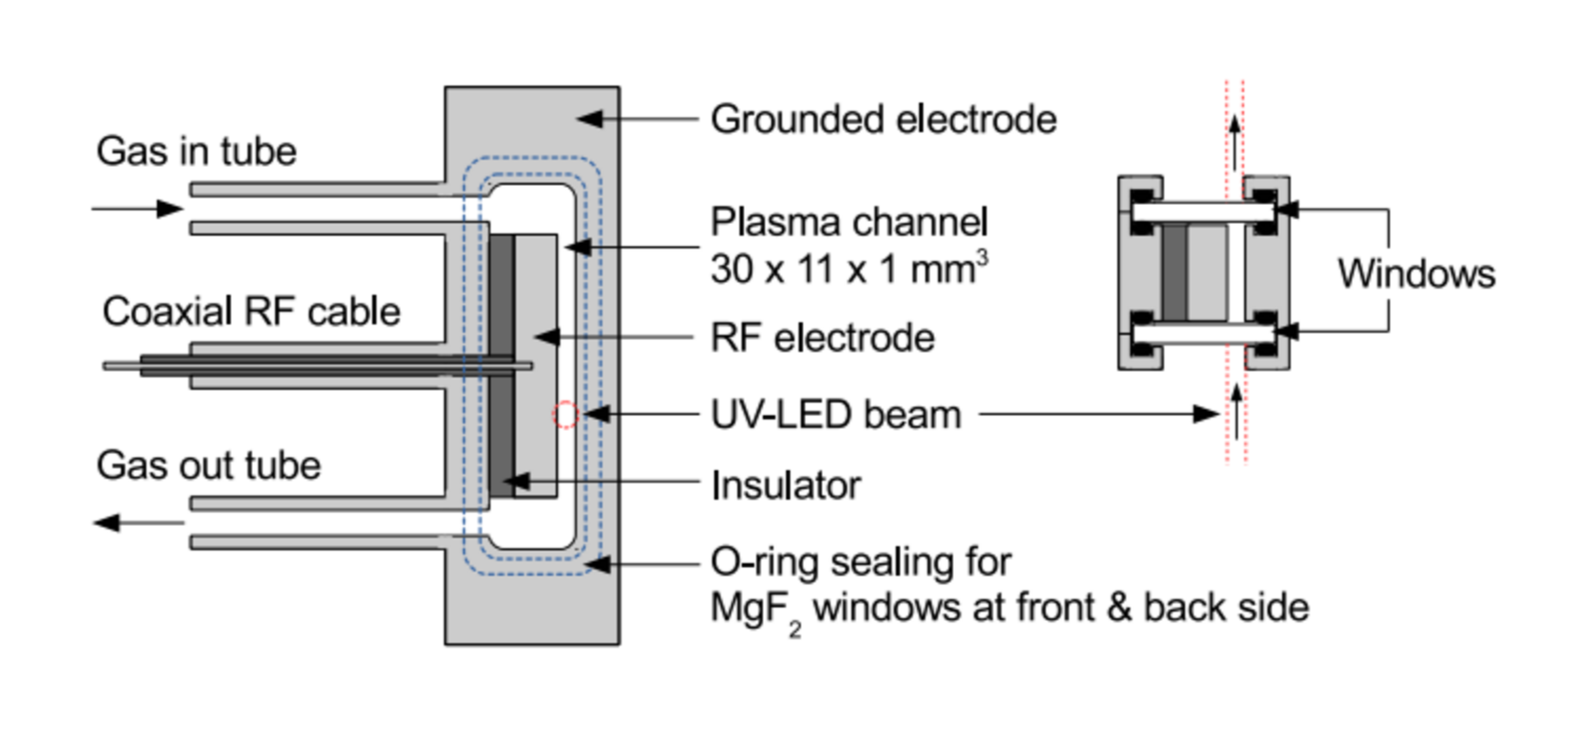
\includegraphics[width=\textwidth]{Figures/PlasmafromApiwat}
	\caption{Diagram showing the RF plasma source from the side (left) and the top (right). Acknowledgements to Apiwat Wijaikhum for provision of the diagram.}
	\label{fig:PlasmaSource}
\end{figure}





%\begin{figure}
   % \centering
   % 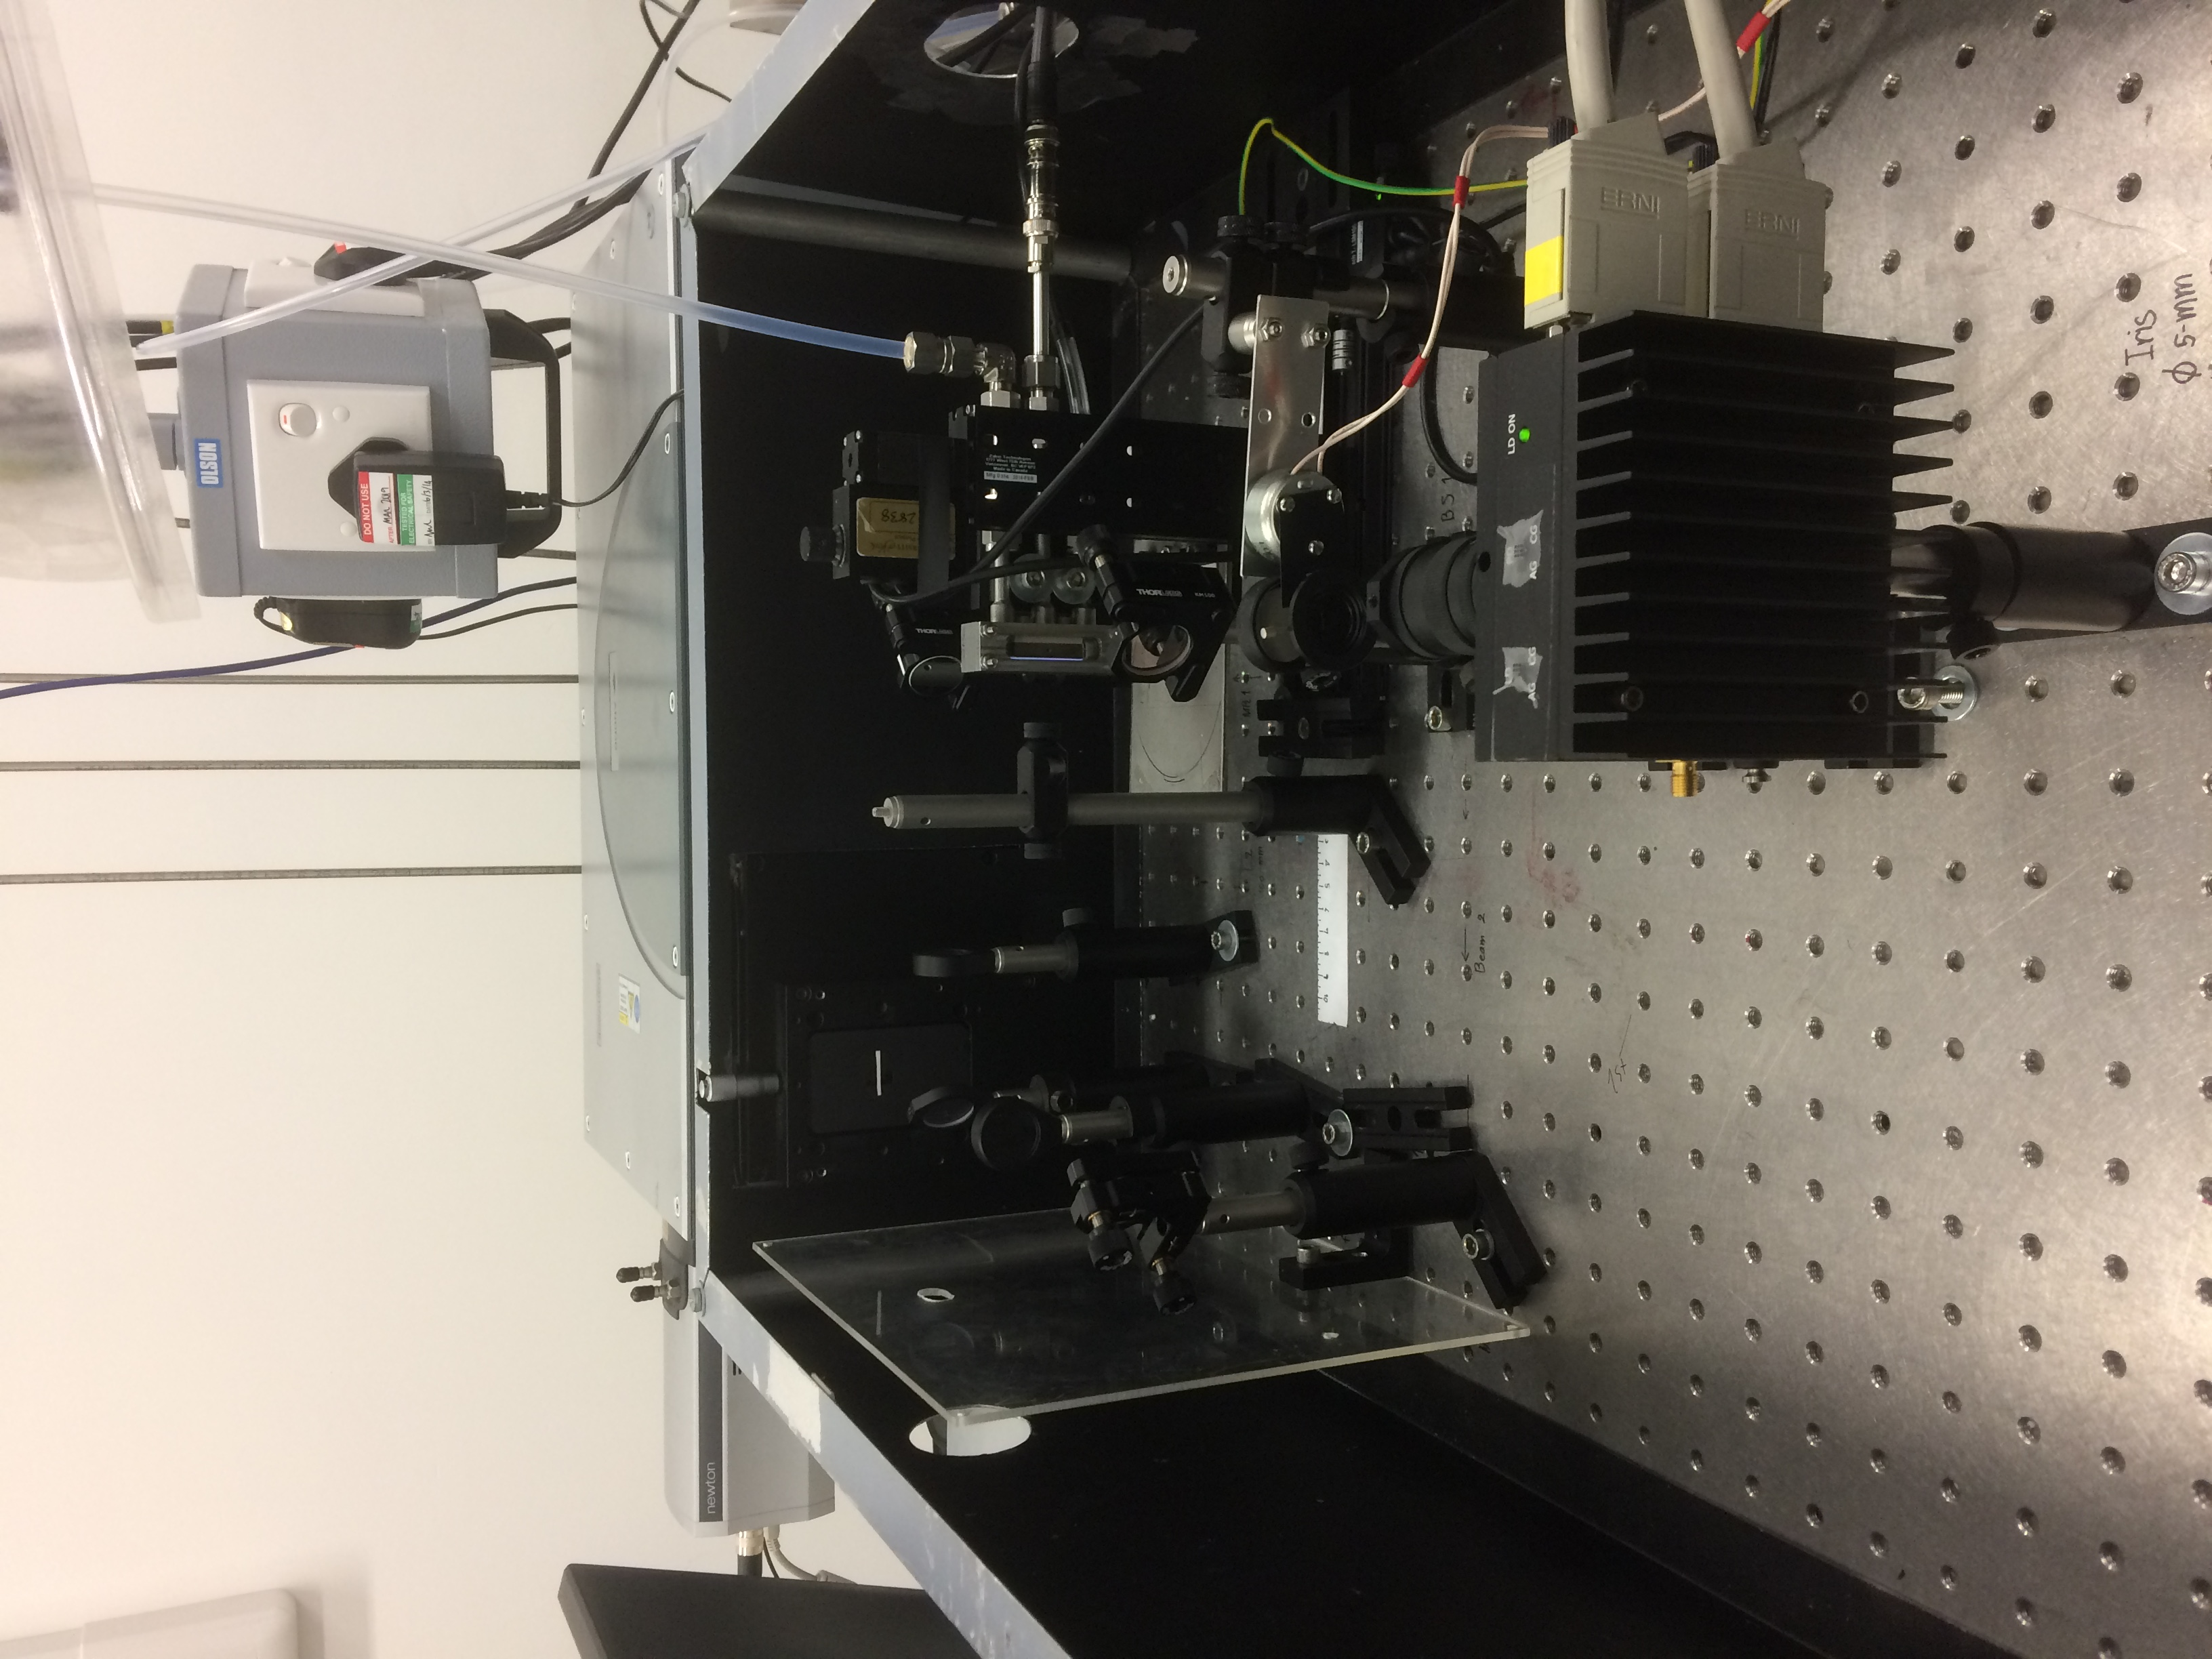
\includegraphics[width=\textwidth]{Figures/PlasmaSetup.JPG}
   % \caption{Plasma Setup...This will be a proper diagram...}
   % \label{fig:my_label}
%\end{figure}


\subsection{Power Measurements}

Whilst the RF generator gives an indication of the power being supplied to the plasma source, it is not very accurate and is unable to account for power losses in cables and other equipment.
To counteract this, the actual power delivered to the plasma can be accurately measured using voltage and current probes connected between the matching box and the plasma source, all connected to an oscilloscope. 
Using these probes, the power supplied to the plasma can be accurately assessed using the equation:

\begin{equation}
P = I \times V \times cos(\theta)
\end{equation}

where $P$ is power, $I$ is current, $V$ is voltage and $\theta$ is the phase difference between the voltage and current.
The challenge with measuring the power supplied to the plasma using this method is accurately measuring the phase difference between the two waveforms as it is usually very small.
It is therefore necessary to use an oscilloscope with a high enough resolution that it's sampling rate is sufficient to be able to tell the phase difference.
A capacitor with a known phase difference of 90$^{\circ}$ is used to compare to the voltage and current waveforms to get an accurate measurement of their phase difference.
Measurements are taken firstly with the plasma on, then with the plasma off to calculate power lost in the equipment, then finally with the capacitor connected.
The actual power is then determined by using the equation above then subtracting the background losses (obtained during the plasma off measurements), from the measurements with the plasma on.

%To accurately get power need to accurately get phase difference. This is hard cos oscilloscope only samples at whatever rate and phase difference between voltage and current is very small. Also, with the jets, the phase difference is near to -90 degrees which would mean that cos theta is nearly 0 therefore needs to be accurate as small changes in phase give big changes in power.

%Instead of fitting to the sampled points, do a fast fourier transform which translates the V and I waveforms from time to frequency and also tells you phase difference using capacitor.

%Therefore, to get accurate measurements, need to have a fast oscilloscope and/or lots of cycles recorded in order to do the FFT to get the most accurate power measurements.

Using this, the actual power delivered to the plasma was calibrated to the output stated on the output dial (see figure \ref{fig:OutputDial}) of the RF generator. 
This was done by changing the output from 50 - 200 in steps of 10 on the RF generator output dial.
For this, the plasma was operated with a gas flow of 5 slm helium containing 5400 ppm water.
This calibration is shown in figure \ref{fig:SolaylPower}.
The relationship between the output and actual power showed a linear relationship and by fitting a line to the measured data, the actual power delivered to the plasma for each output value can be predicted using the line with equation y = 0.1127x - 0.0437 fitted to the data.
All powers stated in this report are real powers calculated from this calibration.

\begin{figure}
    \centering
    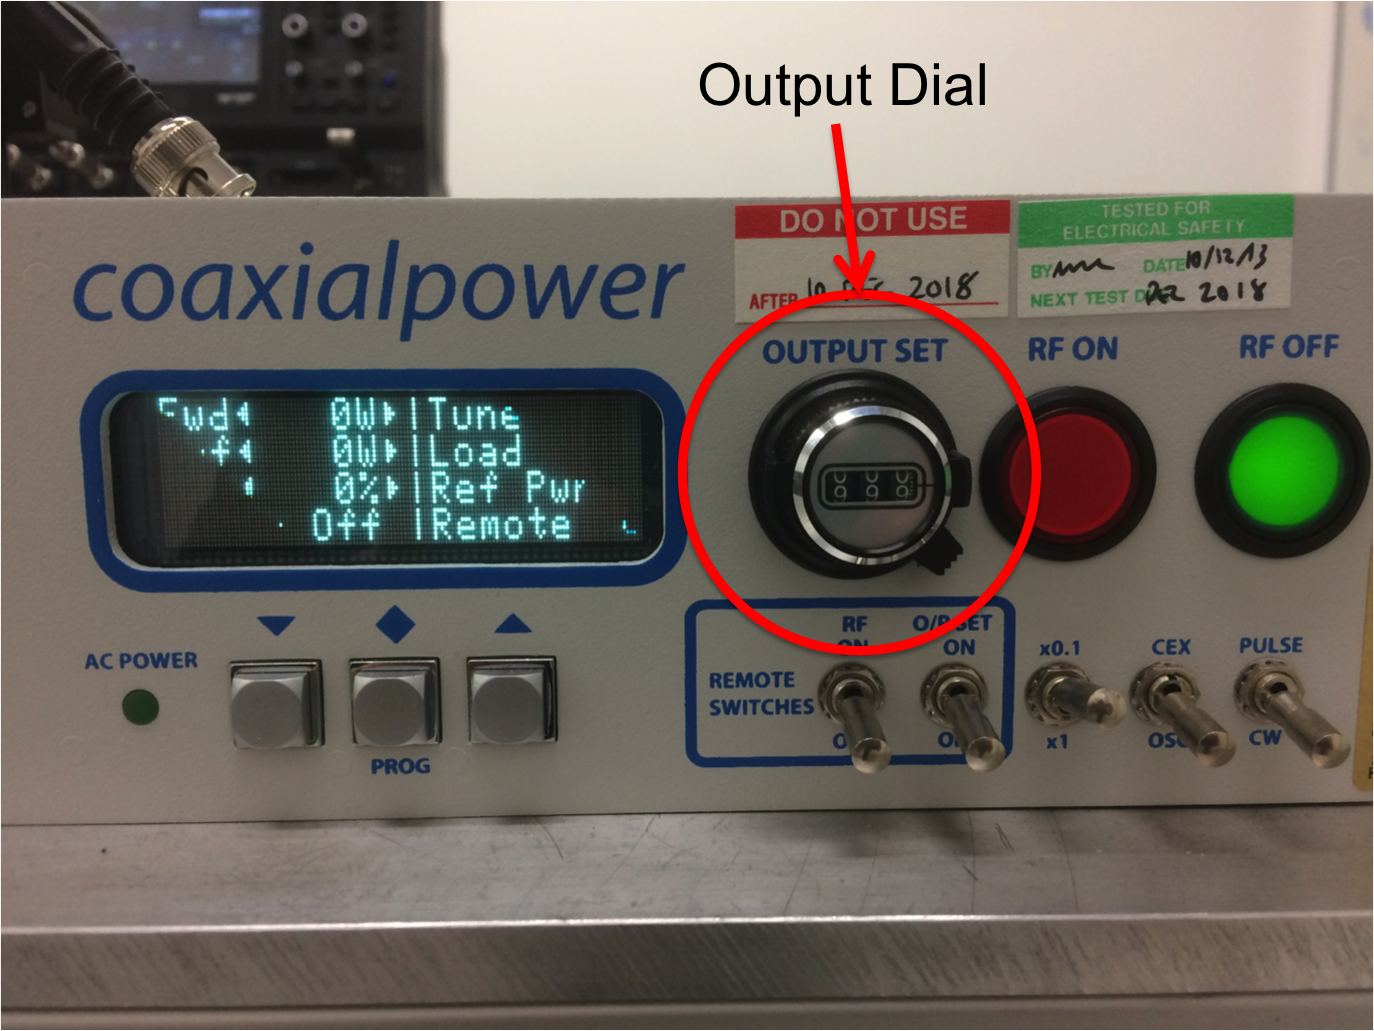
\includegraphics[width=0.4\textwidth]{Figures/OutputDial.png}
    \caption{Picture showing the output dial on the RF generator used for calibrating output from the RF generator to the actual power supplying the plasma}
    \label{fig:OutputDial}
\end{figure}

\begin{figure}
    \centering
    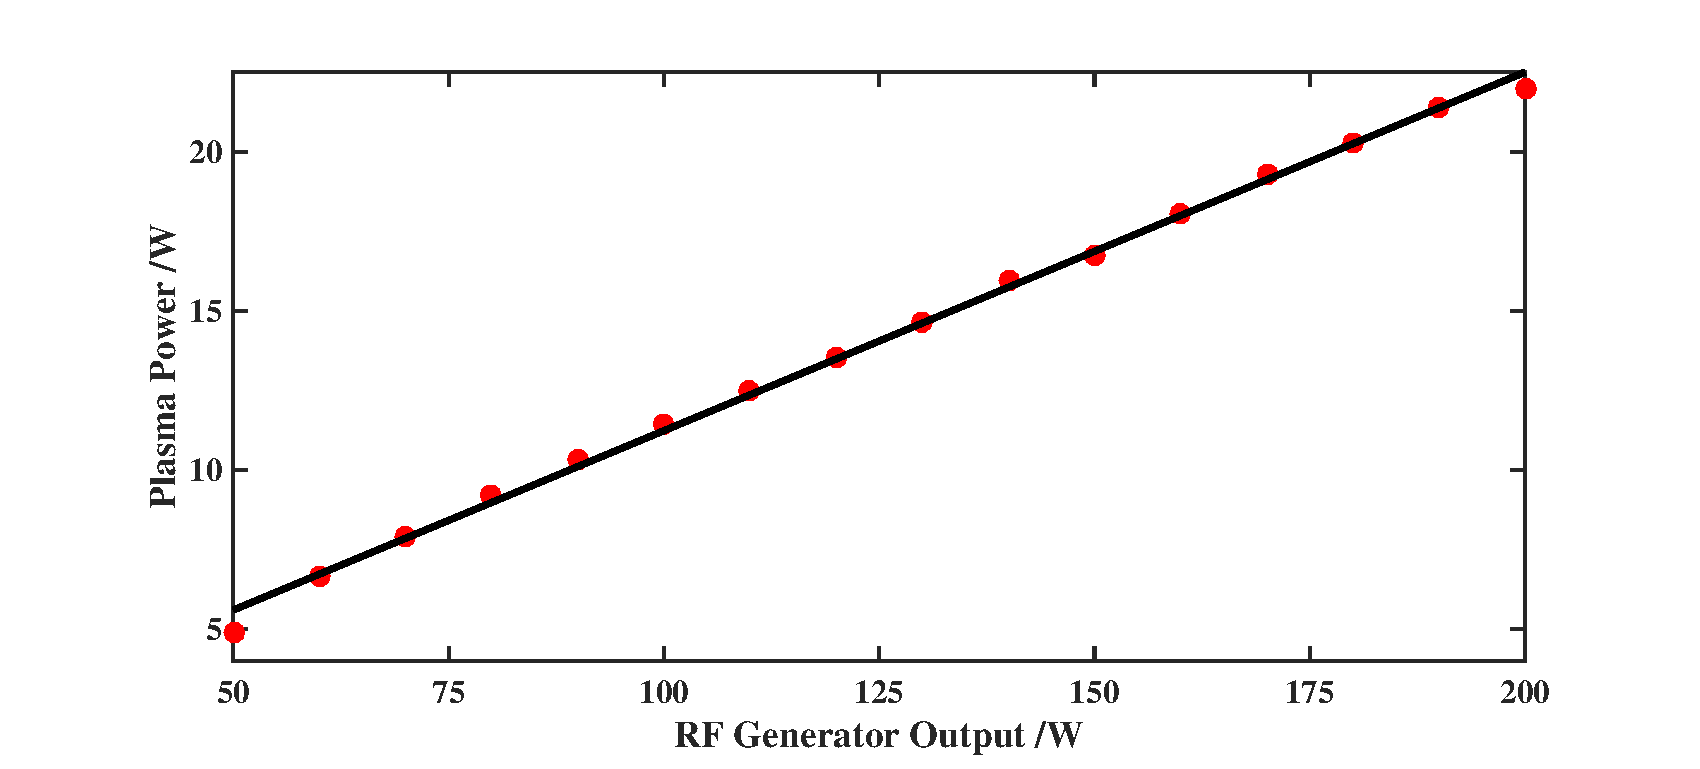
\includegraphics[width=\textwidth]{Figures/ActualPowerBig.eps}
    \caption{Plasma power as a function of RF generator power determined for a helium and 0.54\% water admixture. The line of best fit has the equation y = 0.1127x - 0.0437. The x axis shows the output from the RF generator (see figure \ref{fig:OutputDial}.and the y axis shows the corresponding power in W supplied to the plasma (plasma power) corrected for losses in equipment.}
    \label{fig:SolaylPower}
\end{figure}

Following this calibration, it was necessary to check that the power delivered to the plasma was unaffected by changing the water content of the feed gas by altering the proportion of the 5 slm helium which is passed through the bubbler.
This was checked at two different powers. 
For each power, the RF generator output was kept constant and the volume of helium passing through the bubbler was varied.
The results show that varying the water content has very little, if any effect on the power supplied to the plasma (data not shown).

%\begin{figure}
   % \centering
    %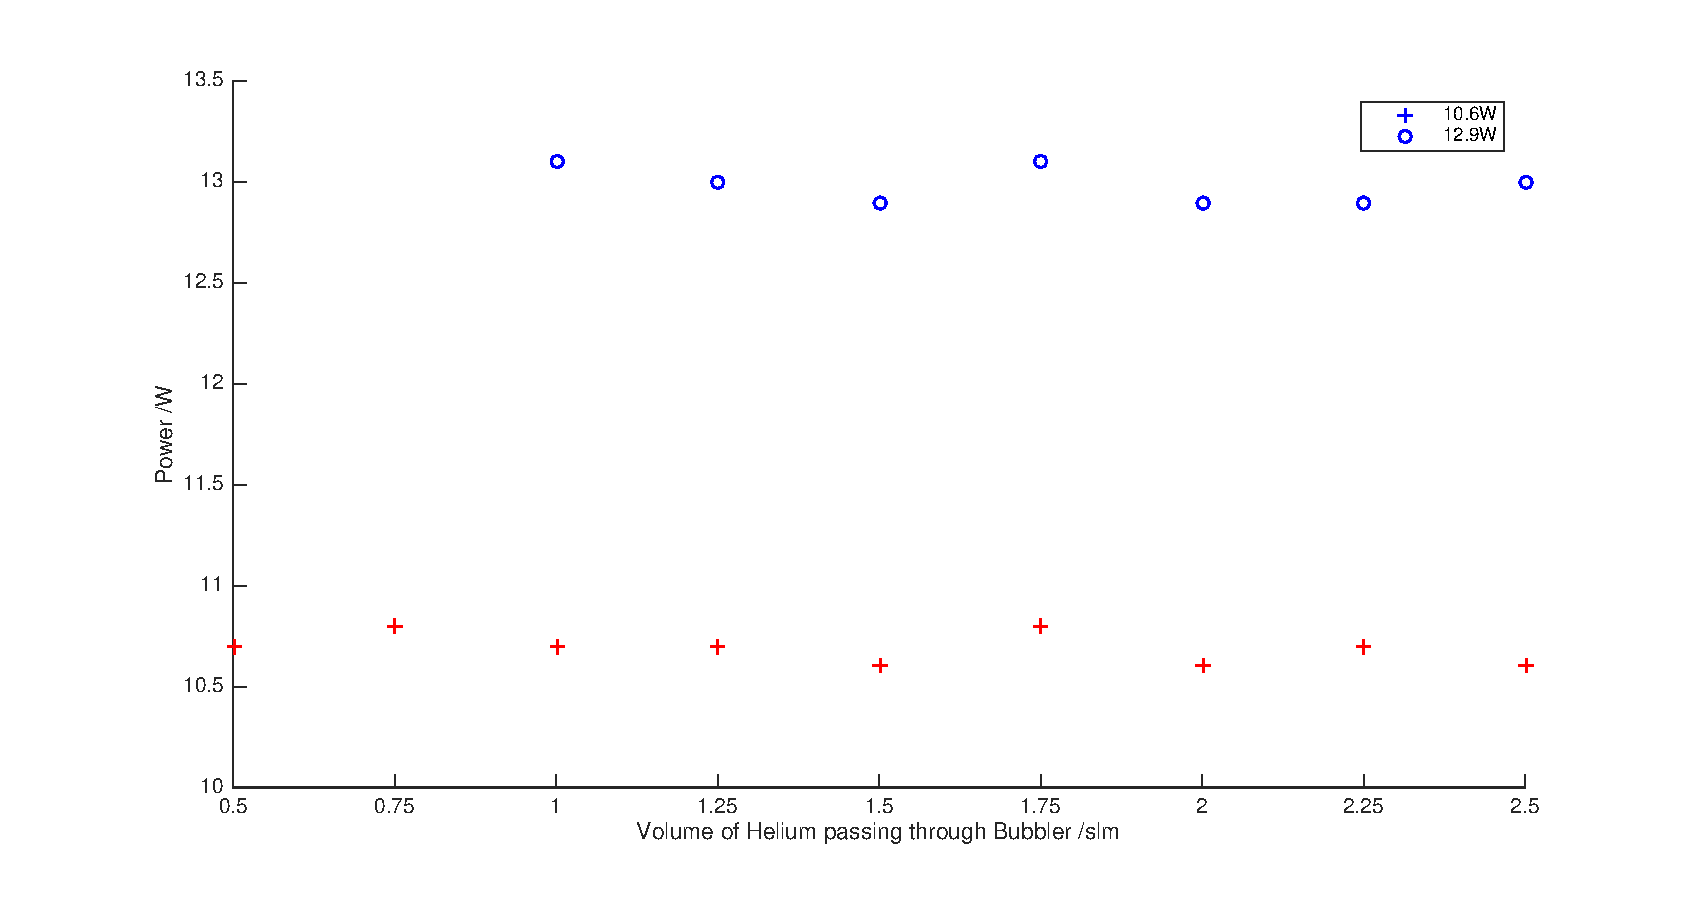
\includegraphics[width=\textwidth]{Figures/BubblerPower.eps}
    %\caption{The water content of the feed gas has no effect on the power supplied to the plasma. The water content of the feed gas was varied at high and low power. For each of the two powers, the output of the RF generator was kept constant and only the water content of the feed gas changed.}
    %\label{fig:BubblerPower}
%\end{figure}

\subsection{UV Absorption Spectroscopy} \label{sec:AbsorptionSpec}

To investigate the density of hydroxyl radicals present in the plasma, absorption spectroscopy was used. An ultraviolet (UV) light emitting diode (LED) with central wavelength of 309 nm was used as this wavelength is specifically absorbed by free hydroxyl radicals \cite{Hatano2010}.
The principle of this method is to measure the intensity of light before and after passing through the plasma, in order to see how much has been absorbed within the plasma by the species of interest \cite{Reuter2015}.
In this case, the species of interest is the hydroxyl radical, therefore, the more hydroxyl radicals present in the plasma, the greater the absorbance of LED.

The absorbance is determined using the Beer-Lambert law, and is therefore dependent on the absorption path length (the distance the light has to travel through the plasma), the absorption cross section of the species (the effective area of the species capable of absorbing light) and the density of the species.

The transmittance of light beam and it's relationship to the absorbance, according to the Beer-Lambert law, is shown as follows:

\begin{equation} \label{eqn:Transmittance}
    T= \frac{I_T}{I_0} = e^{A(\lambda)} = e^{\sigma(\lambda) \cdot L \cdot n}
\end{equation}
Where $T$ is transmittance, $I_T$ and $I_0$ are the intensities of the transmitted and incident light, respectively, $A$ is the absorbance of light by the plasma which is related to the absorbance cross section ($\sigma(\lambda)$), absorption path length ($L$) and the density of the absorbing species ($n$).

The UV beam passes through the plasma and a series of optics, then signal is detected by an imaging spectrograph with a (CCD) camera as shown in figure \ref{fig:Setup}. 
In this setup, there are two LED beams, termed the probe beam, which passes through the plasma source, and the reference beam, which bypasses the plasma.
Both beams enter the spectrograph and are imaged on the CCD but at different vertical positions.
The reference beam allows for a more accurate background measurement and therefore improves the signal-to-noise ratio.
This particular absorption spectroscopy setup built in-house, allows for highly sensitive measurements due to it's two beam nature.
This is particularly important for the spatially resolved densities presented below.

\begin{figure}
	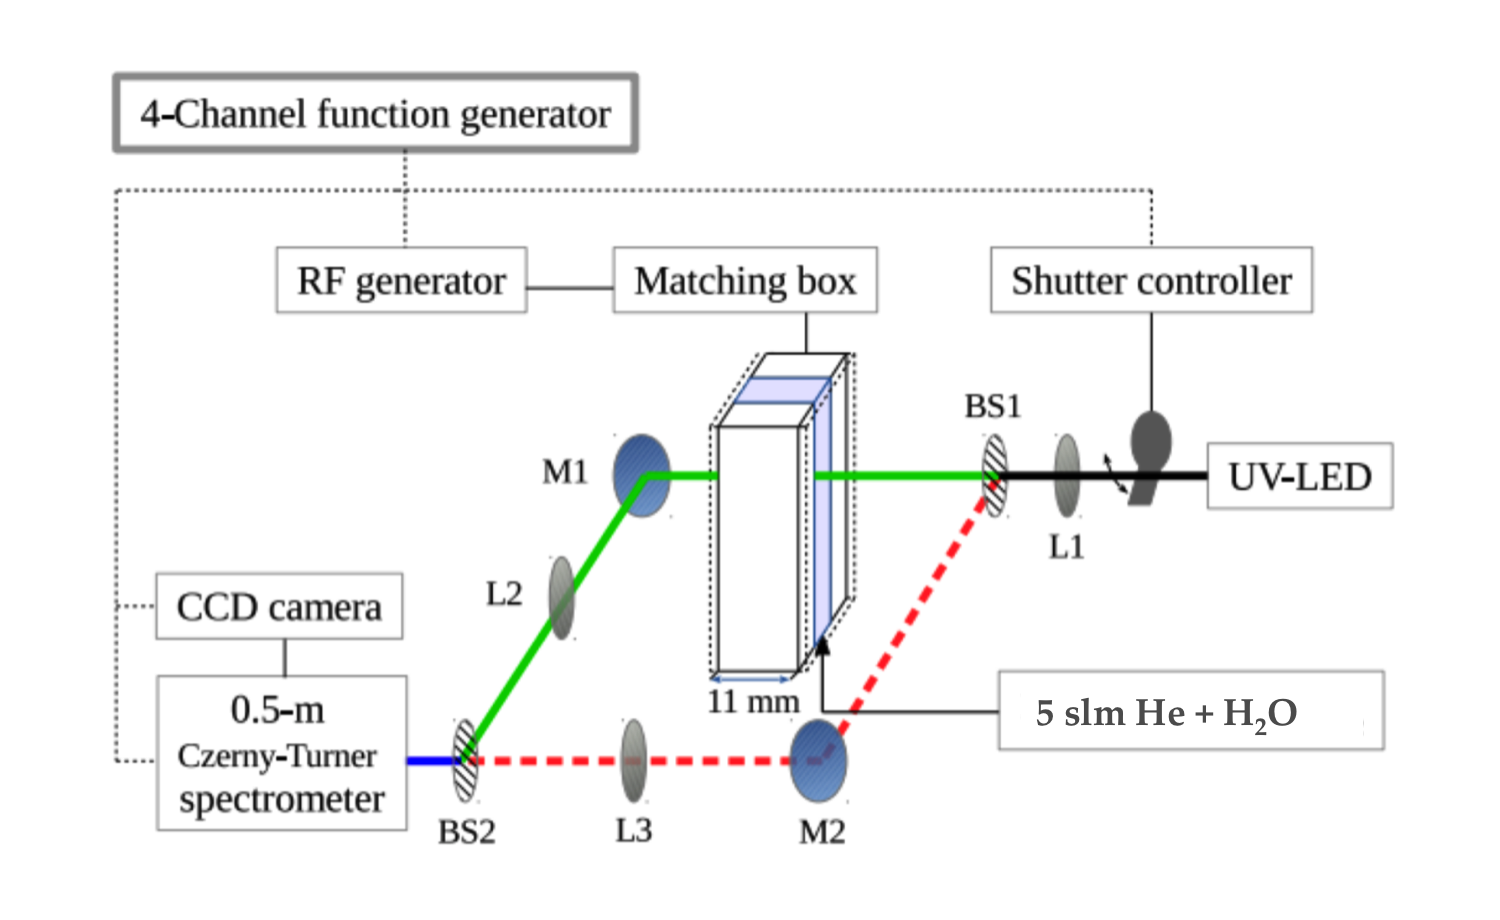
\includegraphics[width=\textwidth]{Figures/SetupfromApiwat}
	\caption{Diagram to show the absorption spectroscopy setup. The probe beam is shown by a solid green line, while the reference beam is shown by a dashed red line. Acknowledgements to Apiwat Wijaikhum for provision of the original diagram, adapted for this particular setup.}
	\label{fig:Setup}
\end{figure} 


In order to measure $I_T$ and $I_0$ for the plasma setup, it is necessary to measure four different parameters as follows:
\begin{itemize}
    \item $I_{PL}$ - The intensity of light reaching the CCD when both the LED and the plasma are on (figure \ref{subfig:Ipl})
    \item $I_{P}$ - The intensity of light reaching the CCD when the LED is off and the plasma is on (figure \ref{subfig:Ip})
    \item $I_L$ - The intensity of light reaching the CCD when the LED is on and the plasma is off (figure \ref{subfig:Il})
    \item $I_{BG}$ - The intensity of background light when both the LED and plasma are off (figure \ref{subfig:Ibg})
\end{itemize}

\begin{figure}
	\begin{subfigure}{0.45\textwidth}
  	  	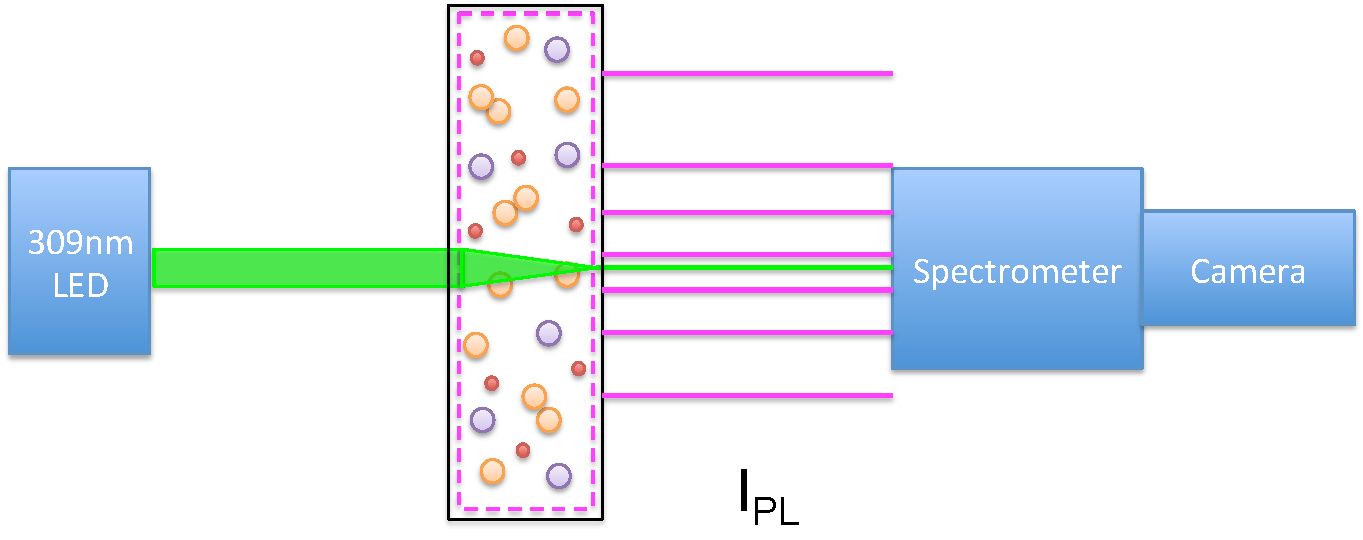
\includegraphics[width=\textwidth]{Figures/Ipl.pdf}
   	 	\caption{$I_{PL}$}
    		\label{subfig:Ipl}
	\end{subfigure}
	\hfill
	\begin{subfigure}{0.45\textwidth}
    		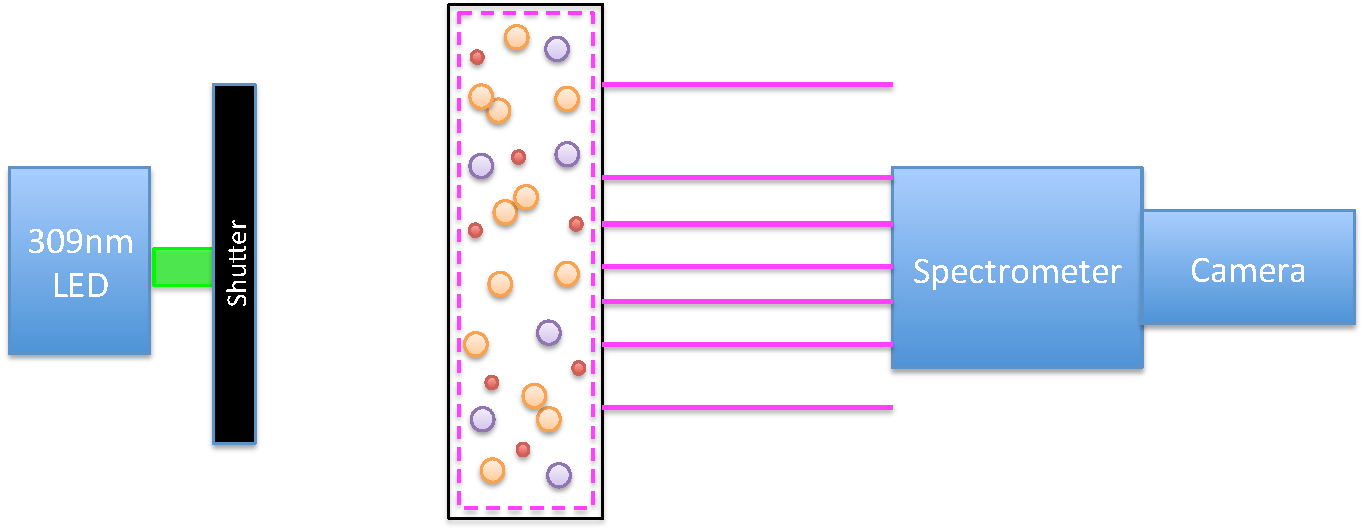
\includegraphics[width=\textwidth]{Figures/Ip.pdf}
    		\caption{$I_{P}$}
    		\label{subfig:Ip}
	\end{subfigure}
	\hfill
	\begin{subfigure}{0.45\textwidth}
		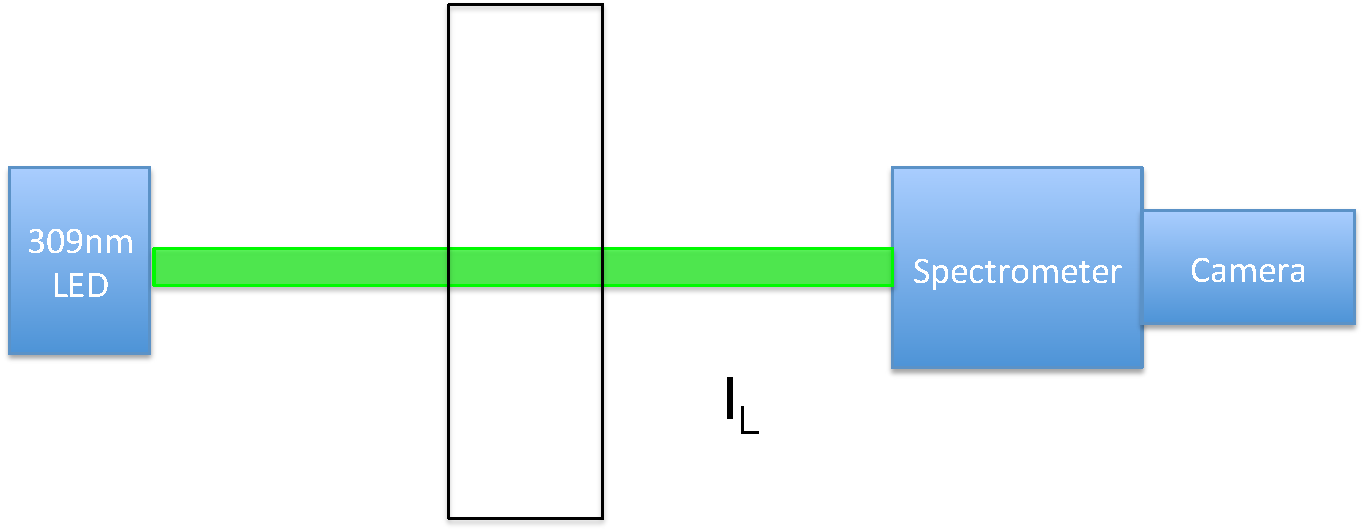
\includegraphics[width=\textwidth]{Figures/Il.pdf}
    		\caption{$I_{L}$}
		\label{subfig:Il}
	\end{subfigure}
	\hfill
    	\begin{subfigure}{0.45\textwidth}
    		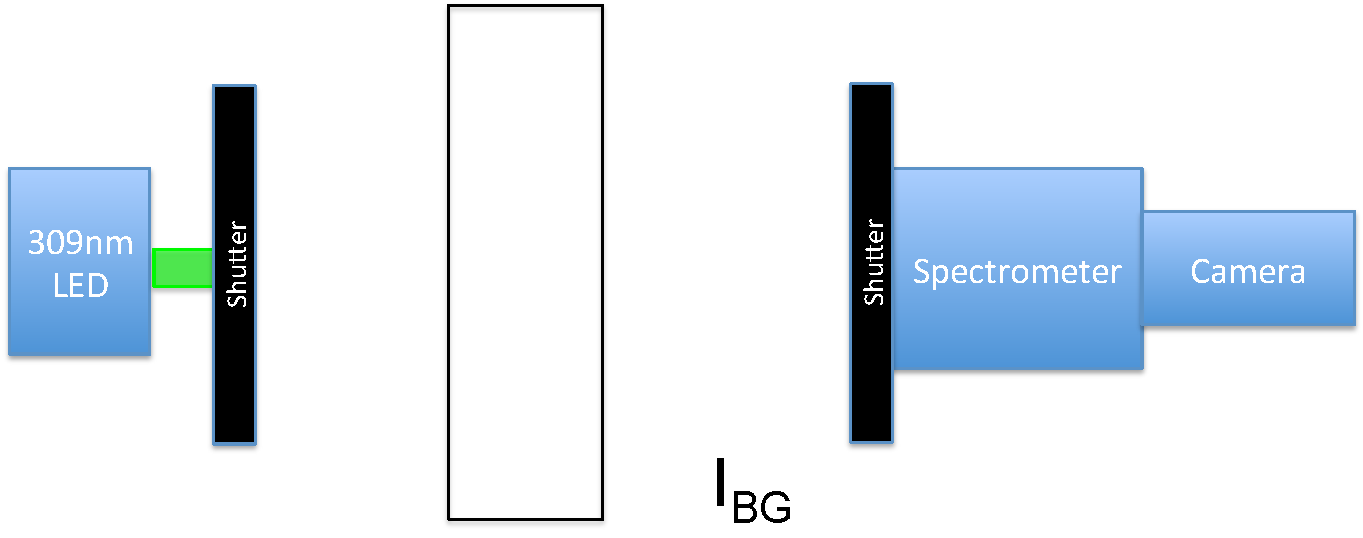
\includegraphics[width=\textwidth]{Figures/Ibg.pdf}
    		\caption{$I_{BG}$}
    		\label{subfig:Ibg}
	\end{subfigure}
	\caption{Diagram showing the different measurements taken to determine absorbance using equation \ref{eqn:Absorbance}, showing the LED (green beam), plasma channel (black rectangle), plasma emission (pink lines), spectrometer, shutters and camera. The pink dashed box denotes the plasma region containing electrons, ions and neutrals (coloured circles).}
\end{figure}

Using these measurements, the equation defining the relationship between transmittance and absorbance becomes:

\begin{equation} \label{eqn:4ParamTransmittance}
    T = \frac{I_T}{I_0} = \frac{I_{PL} - I_P}{I_L - I_{BG}} = e^{-A(\lambda)} = e^{\sigma(\lambda) \cdot L \cdot n}
\end{equation}

All four parameters are measured in series, under the control of a function generator.
This function generator controls a shutter to block the LED and the RF generator to turn the plasma on and off. It also controls external triggering of the camera and a shutter at the entrance to the spectrometer to block all light to the CCD while the system changes from one parameter to the next (see figure \ref{fig:Setup}). 

Data is then acquired as a series of 80 measurements resulting in 20 repeats for each of the four parameters.
Matlab is then used to average all 20 repeats for each parameter then calculate absorbance at each wavelength of the LED as follows:

\begin{equation}\label{eqn:Absorbance}
    A(\lambda) = -ln(\frac{I_{PL} - I_P}{I_L - I_{BG}})
\end{equation}

\subsection{Spectral fitting and radical density determination}

Once the absorbances for each wavelength have been calculated, a simulated spectrum can then be fitted to the data to provide a spectrum of absorbance for hydroxyl radicals (see figure \ref{fig:SpectrumFitting}). 
The spectrum shows absorption due to ground state hydroxyl radicals becoming rotationally and/or vibrationally excited.
In fitting this spectrum, the programme calculates the density of hydroxyl radicals present in the plasma using the absorption cross section of $\cdot$OH and the absorption path length of the plasma, as per equation \ref{eqn:Transmittance}.

\begin{figure}
    \centering
    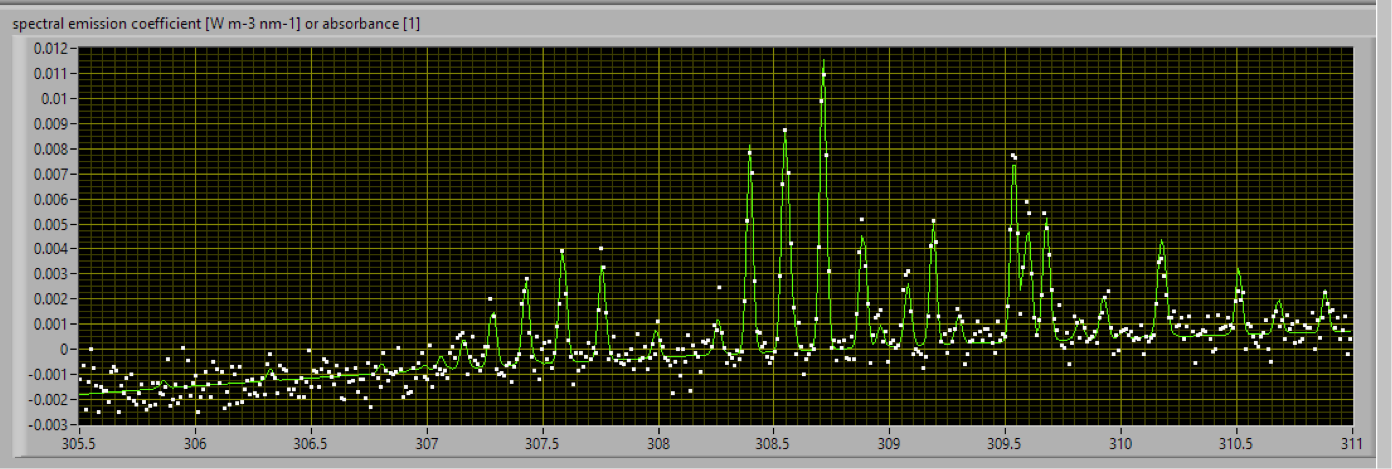
\includegraphics[width=\textwidth]{Figures/SpectrumFitting.png}
    \caption{An example of a simulated spectrum (green line) fitted to the measured absorbances (white dots). Wavelength is shown along the x axis and absorbances along the y axis.}
    \label{fig:SpectrumFitting}
\end{figure}

\subsection{Calculating the Water Content of Helium}
\label{subsec:CalculatingWaterContent}


To calculate the water content of helium passing through the bubbler, firstly, the flow of water must be determined. For this, the pressure of water vapour in the bubbler ($P_{water}$) is calculated using the following equation taken from reference \cite{Alduchov1996}:

\begin{equation}
	e_w = 6.1094 e^{\frac{17.625t}{243.04 + t}}
\end{equation}
Where $e_w$ is the water vapour pressure in hPa, above a plane surface of pure water, and $t$ is the temperature in degrees celsius.

The pressure of helium ($P_{He}$) is taken to be $P_{atmosphere} - P_{water}$. Since the ratio of flow to pressure for helium must be the same as for water, the flow of water can be calculated as follows:

\begin{equation}
    F_{water} = \frac{F_{He} * P_{water}}{P_{He}}
\end{equation}

Where $F_{water}$ and $F_{He}$ are the flows of water and helium in slm, respectively. The percentage of gas flow that is water, and the concentration of water in parts per million can then be determined.
The relationship between the flow of helium through the bubbler and the concentration of water in ppm is shown in figure \ref{fig:WaterContent}.

\begin{figure}
    \centering
    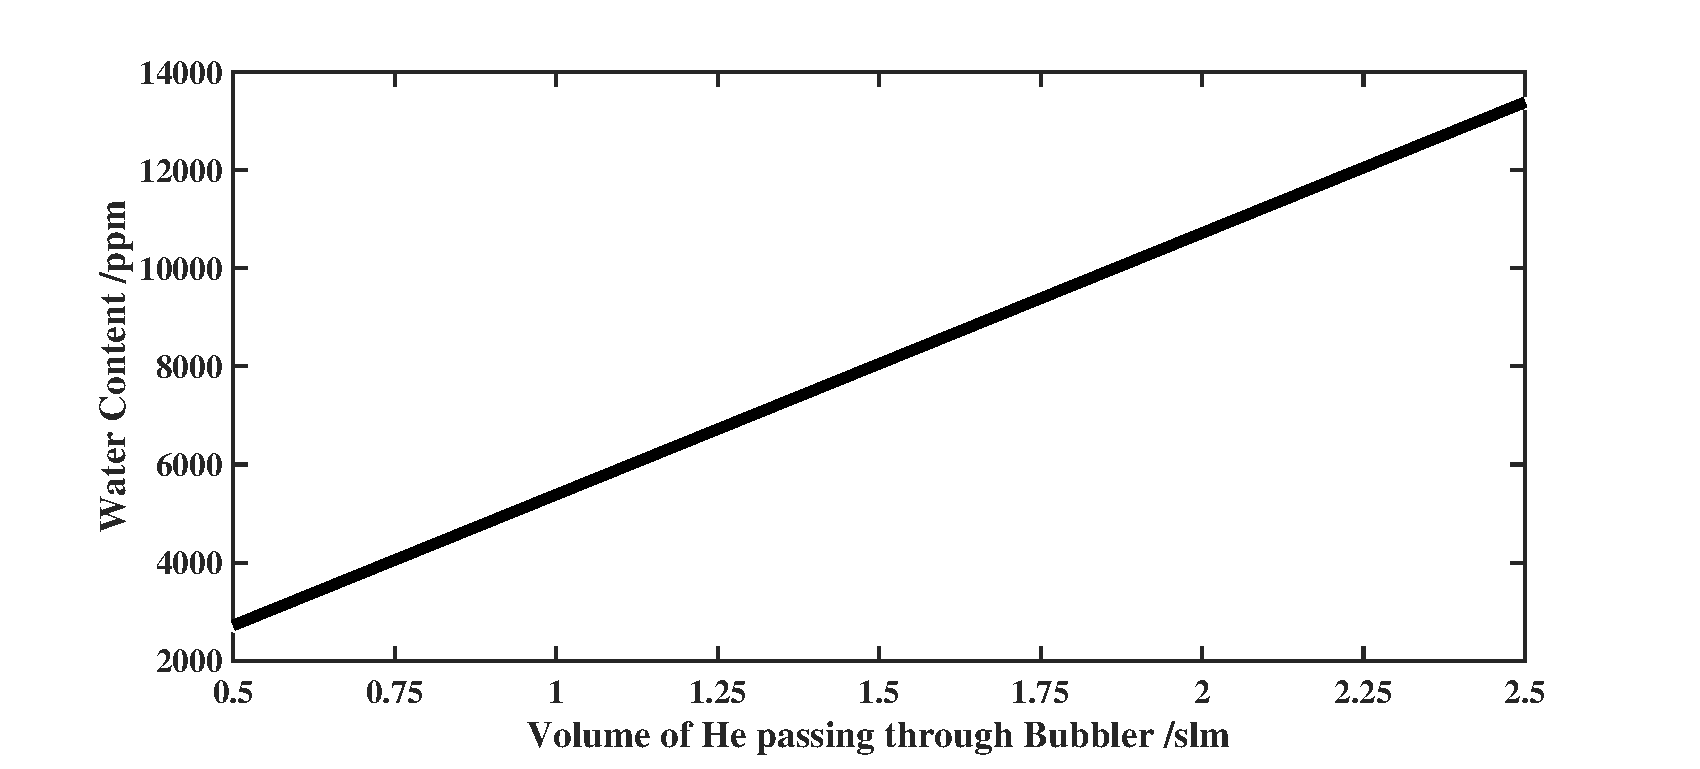
\includegraphics[width=\textwidth]{Figures/WaterContentBig.eps}
    \caption{The water content of the helium passing through the bubbler increases linearly with the volume of helium passing through the bubbler. Water content calculated using equation from \cite{Alduchov1996} and procedure described in the text.}
    \label{fig:WaterContent}
\end{figure}

%\subsection{Modelling of Hydroxyl Radical Production}

%\begin{itemize}
%\item Global model of plasma written by Sandra
%\item approximately 300 reactions taken into account and the probabilities that they will occur
%\item Coupled with gas flow rate, power, plasma volume and diffusion length
%\item Solves equations that take into account the probabilities of species being produced the different reactions (using the rate constants for each reaction), along with the rates of losses due to recombination.
%\item The data from the model can be compared to the experimental data
%\item Running the model then can give an indication of the dominant reactions for the production and loss of hydroxyl radicals
%\end{itemize}



\section{Results}

\subsection{Increasing the power to the plasma increases hydroxyl radical density}

Following investigation of the spatial resolution of hydroxyl radicals, the effects of power variation were then investigated.
It was of interest to see how varying the power would affect the density of hydroxyl radicals and the percentage dissociation of water to hydroxyl.
The 20mm position was chosen to investigate as at this point, the $\cdot$OH densities seem to be at steady state. 
The full range of powers for the plasma were tested from 6.5W (minimum power for sustaining the plasma) to 10.9 W (maximum power before arcing occurs) and results of this are shown in figure \ref{fig:PowerVariation}.

The results show that the density of $\cdot$OH increase non-linearly with increasing power being supplied to the plasma, with a density range of approximately 3.25 - 4.5 x 10\textsuperscript{20} m\textsuperscript{-3}.
The experiment was repeated four times, meaning that a mean and standard deviation could be calculated from the data and is shown in the figure. 
This also gives an indication of the expected error in the experiment which is approximately $\pm$ 0.5 x 10\textsuperscript{20} m\textsuperscript{-3}.

\begin{figure}
    \centering
    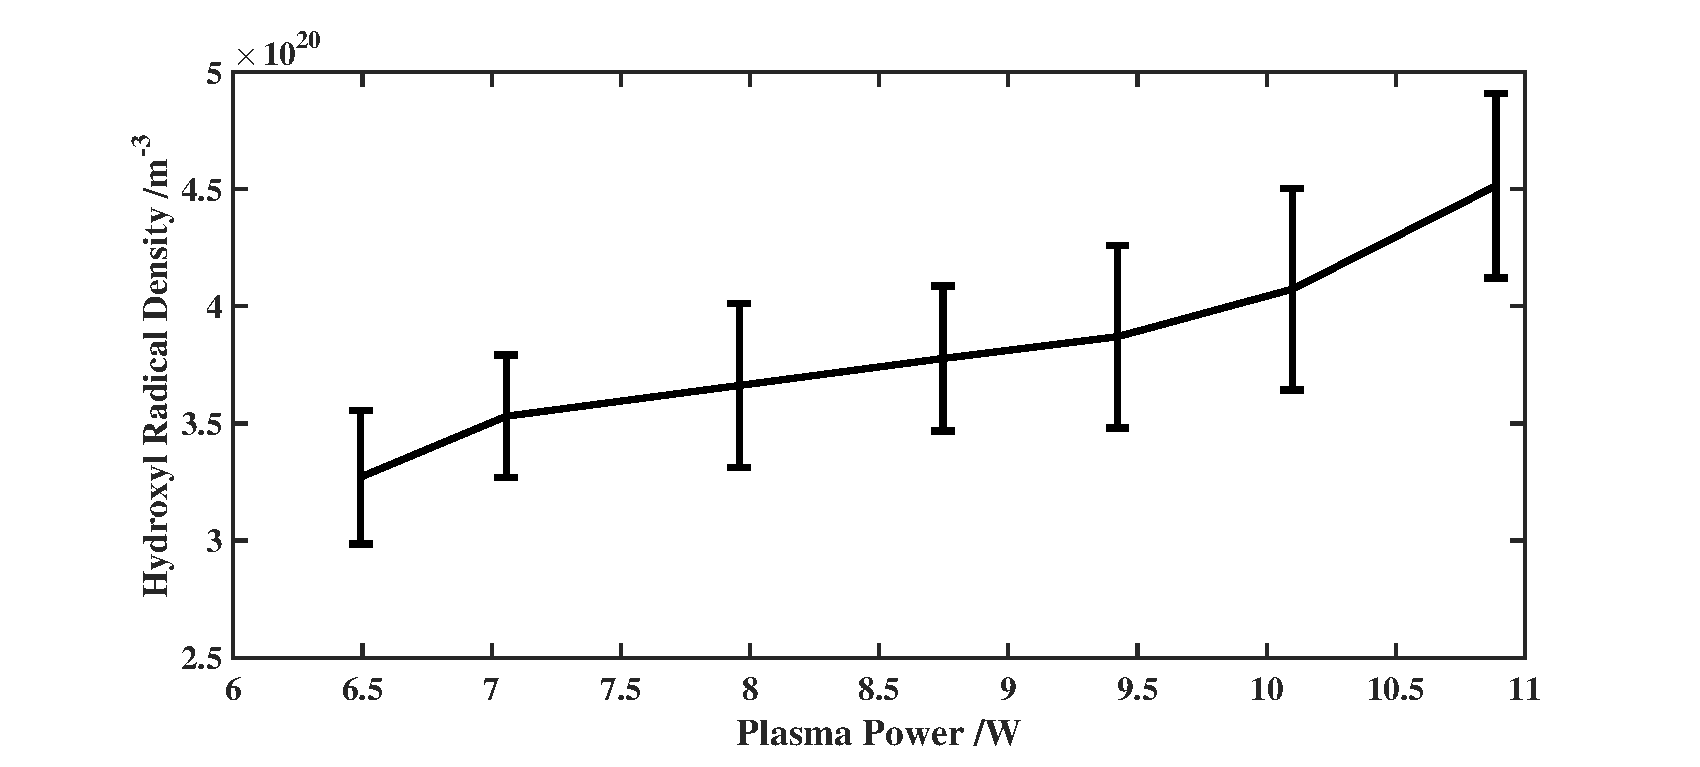
\includegraphics[width=\textwidth]{Figures/PowerVariationBig.eps}
    \caption{Power increases $\cdot$OH density in the plasma region in a non-linear manner. Absorption spectroscopy was performed at a point 20mm from the gas inlet while power being dissipated in the plasma was varied within the range of 6.5 - 10.9 W, as shown on the x axis. Total gas flow to the plasma was kept constant at 5 slm helium with 5400 ppm water. The experiment was repeated four times. The graph shows the average density (shown on the y axis in m\textsuperscript{-3}) for each power and the error bars represent one standard deviation.}
    \label{fig:PowerVariation}
\end{figure}


\subsection{Increasing the water content of the plasma gas feed increases hydroxyl radical density}

To investigate whether increasing the water being fed to the plasma increases the hydroxyl radical density, the ratio of dry and humid helium entering the plasma channel was altered by changing the proportion of the total 5 slm helium that passed through the bubbler. The range of water concentrations entering the plasma was approximately 2700 - 13400 ppm. The results are shown in figure \ref{fig:BubblerVariation}.

The powers had to be carefully chosen due to the effects of adding in additional molecules into the plasma which can act as energy sinks when they absorb energy to change rotational and vibrational states. 
Therefore, higher water contents require higher powers to ignite as the system becomes less efficient when more molecules are added.
Two different powers were used to investigate the effects of altering the water content. Firstly, 8.7W was used as this was sufficient to sustain the plasma at high water contents, without causing arcing at low contents. Secondly, the power was increased to 10.9W to see how the density increased at the higher power. 

The results shown in figure \ref{fig:BubblerVariation} show that $\cdot$OH density increases when the water content of the feed gas increases. This is not unreasonable as we can expect the main $\cdot$OH production mechanism to be electron impact with water (further discussed in section \ref{subsec:SpatialRes}, therefore the more water present, the greater the $\cdot$OH production.
For both powers, the $\cdot$OH density initially increases with increasing water content and then starts to saturate.
This may be due to either a less effective production mechanism at higher water admixtures or a competing $\cdot$OH consumption mechanism.

%However, particularly at the lower power, it appears that the densities increase fairly quickly between approximately 2500 - 7000 ppm of water, before starting to level off.
%This would suggest that maybe lower water contents would be interesting to investigate?

\begin{figure}
    \centering
    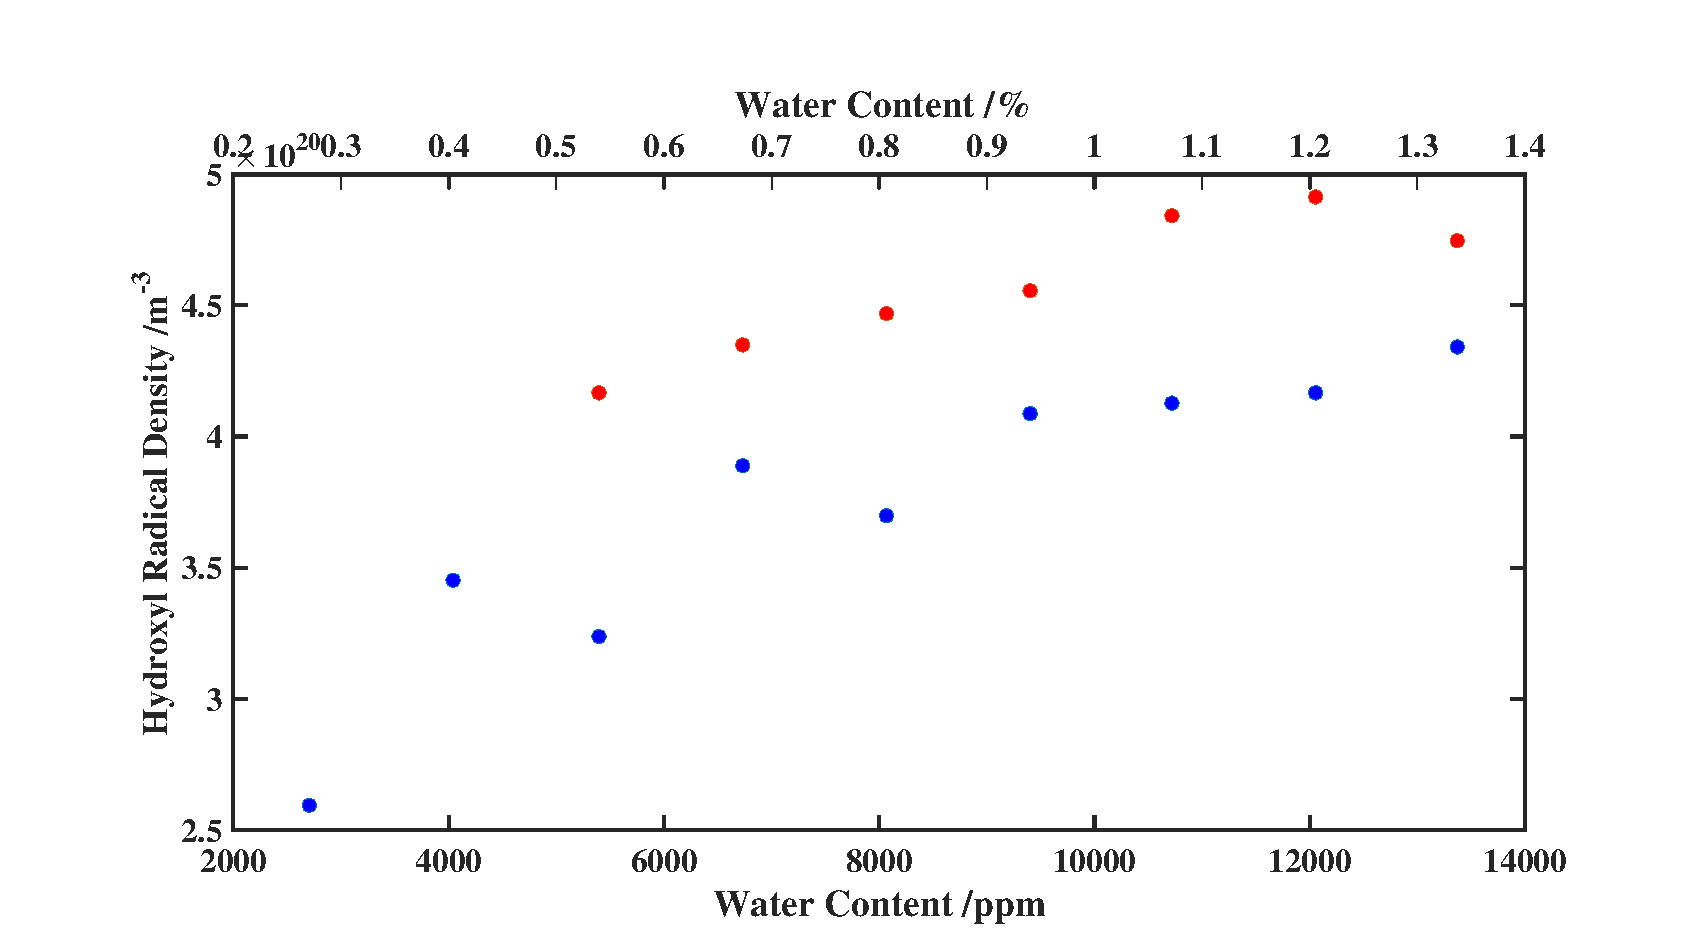
\includegraphics[width=\textwidth]{Figures/BubblerVariationBig}
    \caption{Increasing the water content of the plasma feed gas increases $\cdot$OH density in the plasma. Absorption spectroscopy of the plasma was performed at 20mm from the gas inlet to determine $\cdot$OH density (shown on the y axis). A total gas flow of 5 slm was maintained throughout, with differing water contents, ranging from 2700 - 13400 ppm (shown on the x axis). The powers used were 8.7W (blue dots) and 10.9W (red dots)}
    \label{fig:BubblerVariation}
\end{figure}


\subsubsection{Percentage Dissociation}

The degree of dissociation of water to hydroxyl radicals was then investigated by comparing the concentration of water entering the plasma, with the concentration of $\cdot$OH in the plasma.
The percentage dissociation is calculated as follows:

\begin{equation} \label{eqn:PercentDiss}
	\frac{concentration \cdot OH}{concentration  H_2O} \times 100
\end{equation}

The results of this calculation for each of the water contents measured are shown in figure \ref{fig:BubblerDissociation}.
Firstly, the results show that the percentage dissociation of water to $\cdot$OH is very small (\textless 0.4\%). This may be due to the very highly reactive nature of $\cdot$OH which means that it is destroyed very shortly after being created therefore is, very quickly, undetectable.
Secondly, the graph shows that the percentage dissociation decreases as the water content increases, for both the low and high power.
This is more surprising due to the fact that the opposite is seen when considering $\cdot$OH density (see figure \ref{fig:BubblerVariation}).
However, the decrease in percentage dissociation could be explained by the fact that increasing the water content of the plasma, increases the number of molecules present which, in turn, decreases the efficiency of the system.
The increase in water content means that more of the energy in the plasma system can be absorbed by the molecules in rotationally and vibrationally excited states.
This results in less energy available for electron processes such as dissociation, electronic excitation and ionisation (see section \ref{section:LowTempPlasmas}), seen here by a decreased dissociation of water.
%Adding in oxygen





\begin{figure}
    \centering
    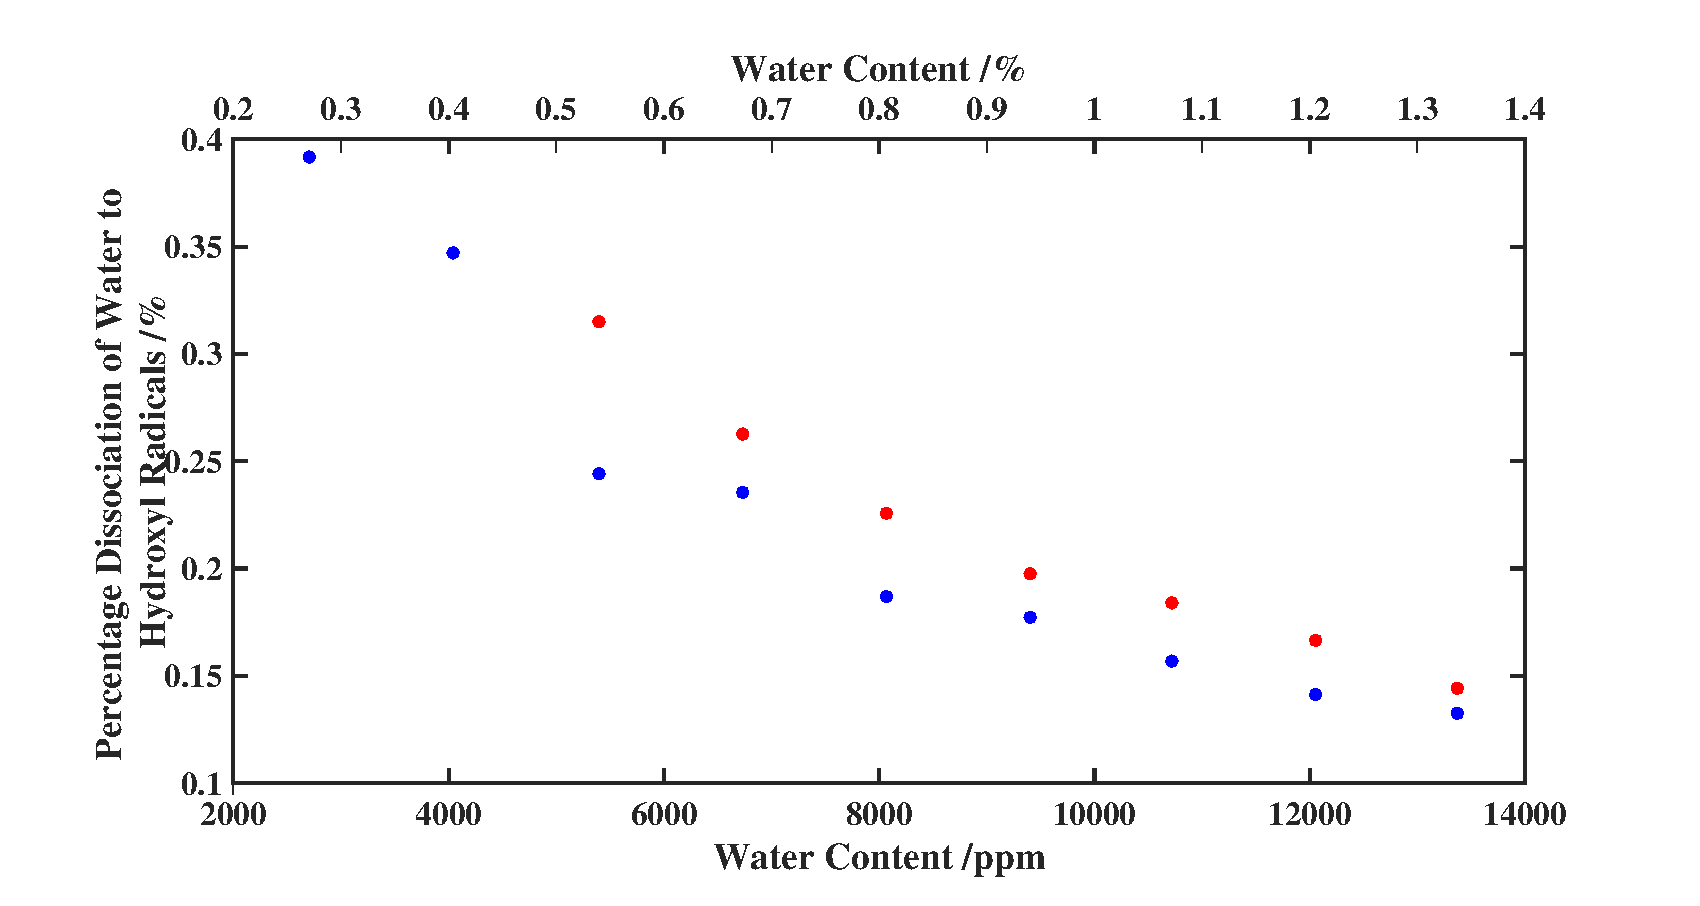
\includegraphics[width=\textwidth]{Figures/BubblerDissociationBig.eps}
    \caption{The percentage dissociation of water to hydroxyl radicals decreases as the water content increases. Absorption spectroscopy was carried out at a point 20mm from the gas inlet. The plasma was operated with a total of 5slm helium with water contents of 2700 - 13400 ppm. The experiment was repeated at two different powers of 8.7 W (blue dots) and 10.9 W (red dots).}
    \label{fig:BubblerDissociation}
\end{figure}


\subsection{Spatial Resolution of Hydroxyl Radicals} \label{subsec:SpatialRes}

\begin{figure}
    \centering
    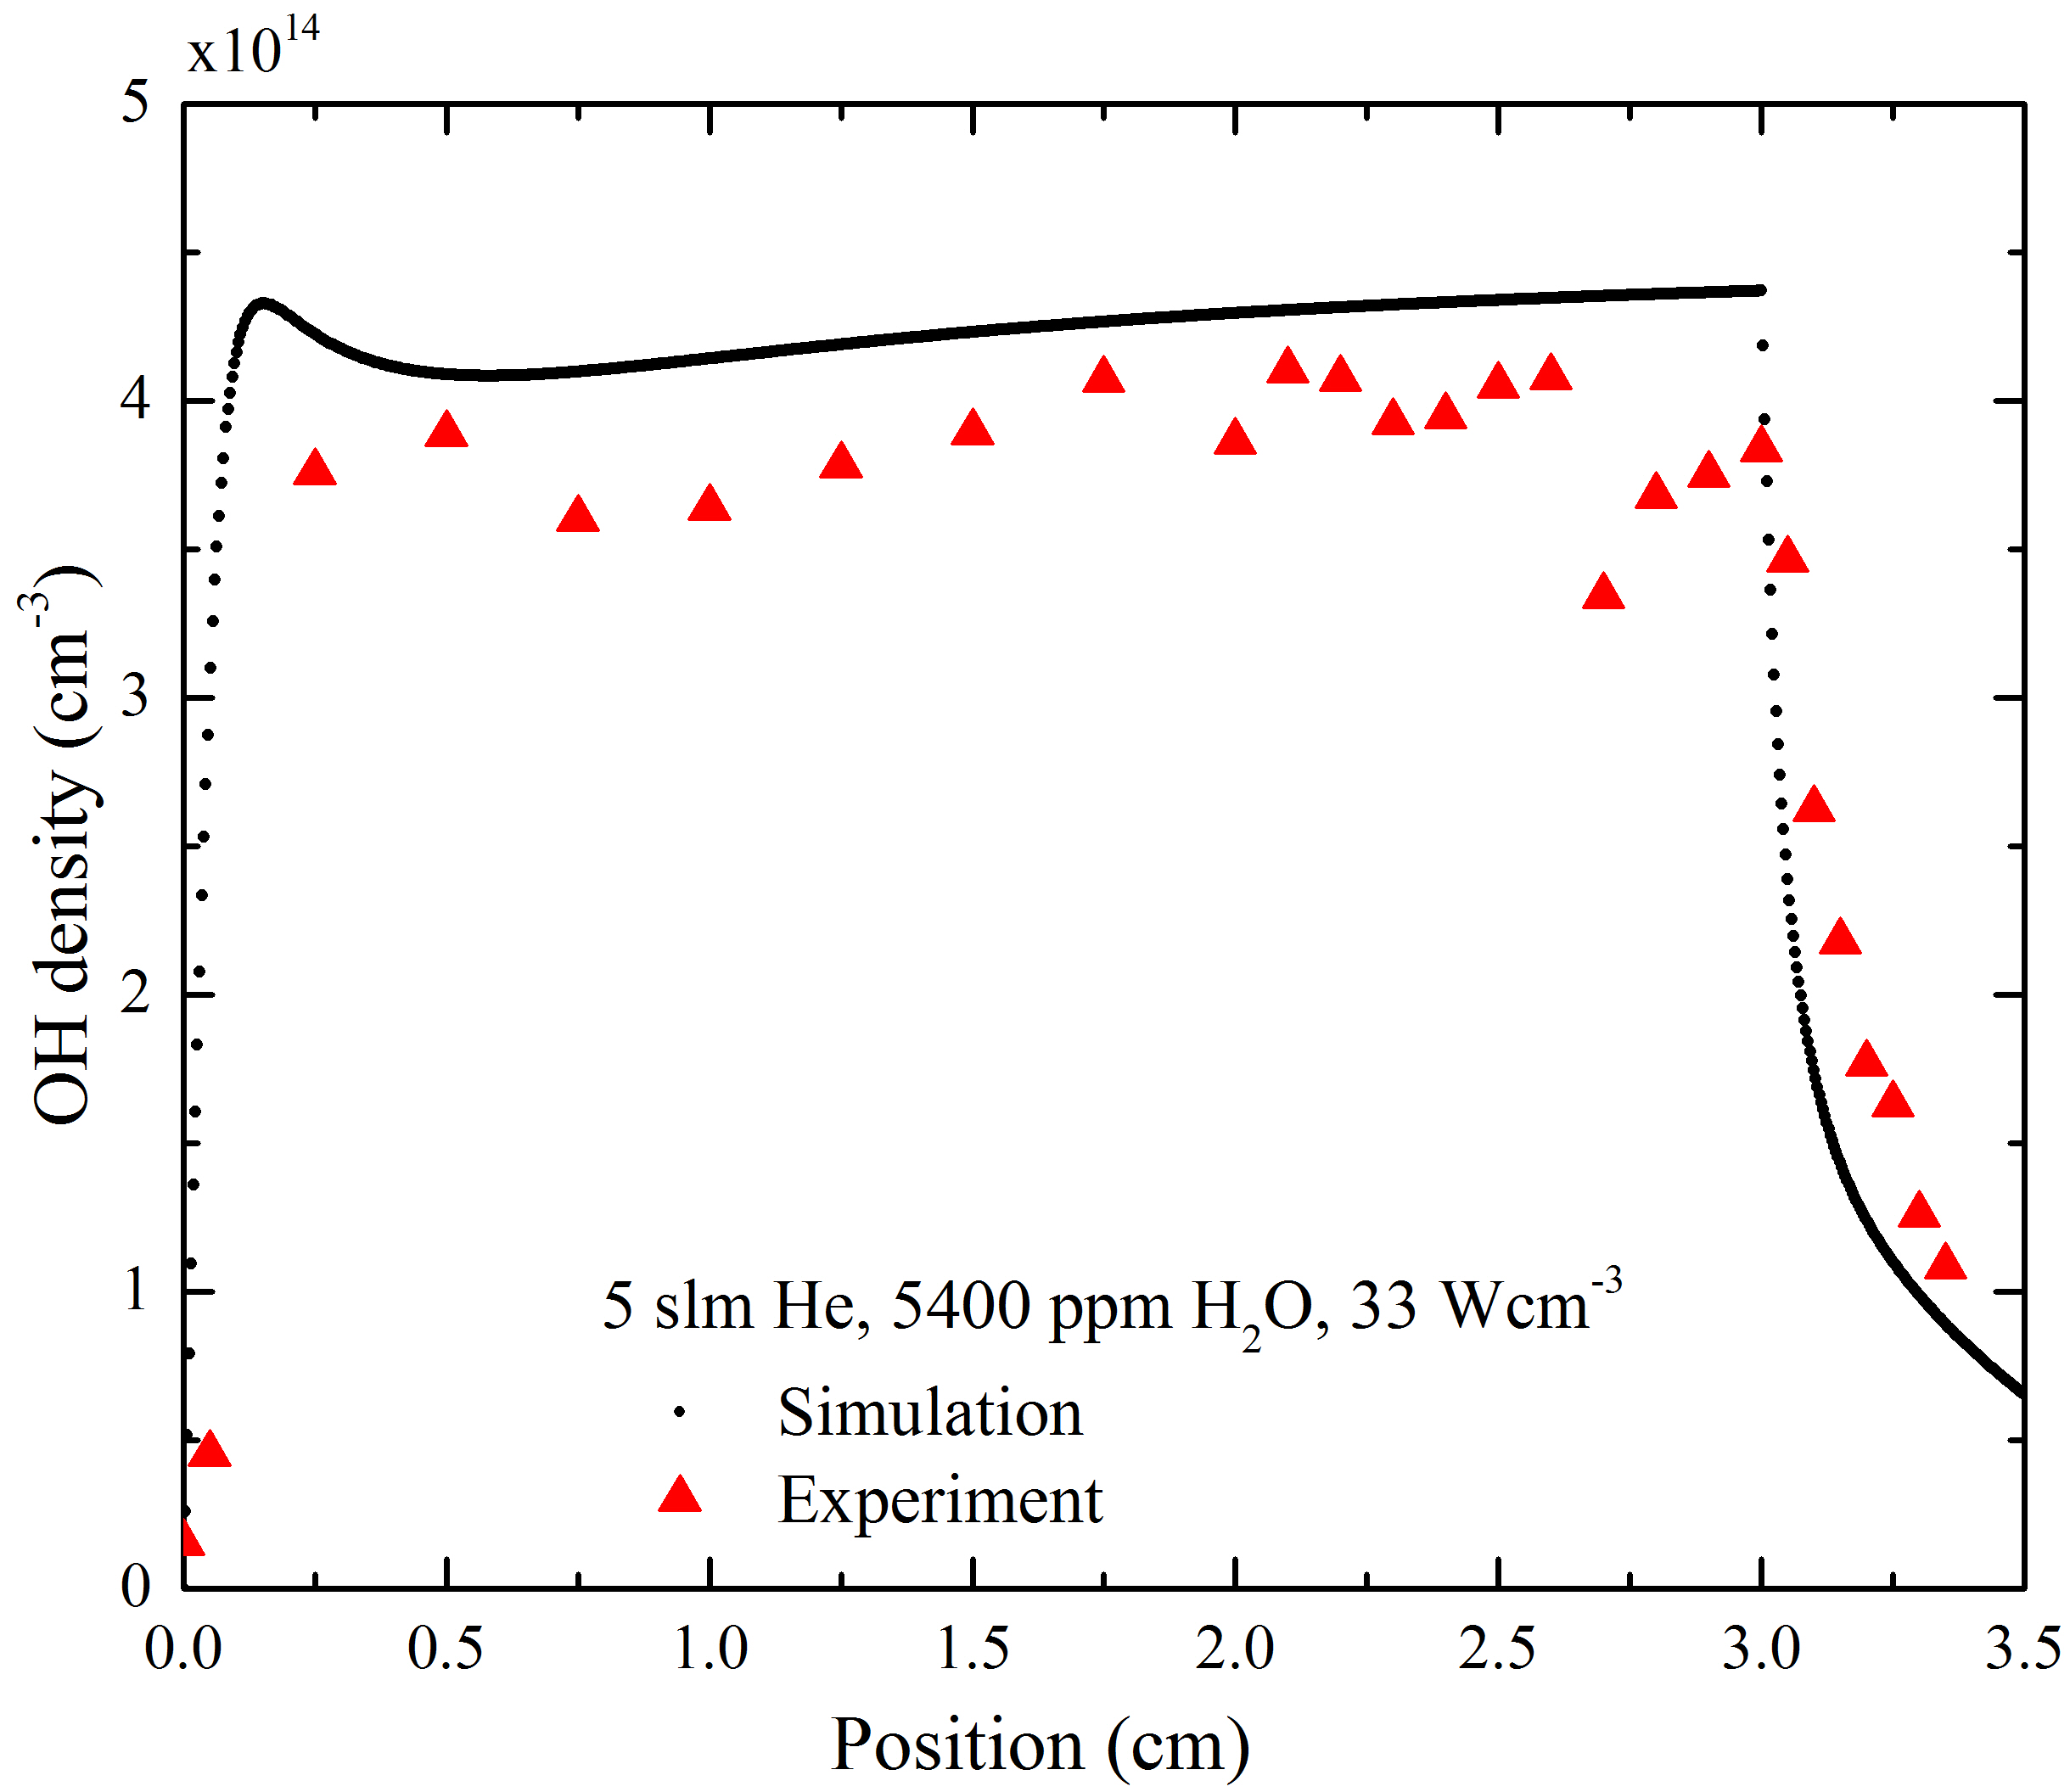
\includegraphics[width=\textwidth]{Figures/OHSpatialwithSimReal}
    \caption{Figure showing $\cdot$OH density as a function of distance along the plasma channel from the gas inlet. Absorption spectroscopy was performed at 0.5 - 1 mm intervals along the 30 mm length of the electrodes (0-30 mm), plus at 0.5 mm intervals beyond the end of the plasma region (30.5-33.5 mm). The position along the plasma channel in mm is shown on the x axis, and the corresponding $\cdot$OH density is shown in m\textsuperscript{-3} on the y axis. The plasma was operated at 10.9 W with a feed gas flow rate of 5 slm with 5400 ppm water. Red triangles denote experimental data, black points show simulated data.}
    \label{fig:SpatialRes}
\end{figure}

\begin{figure}
	\centering
	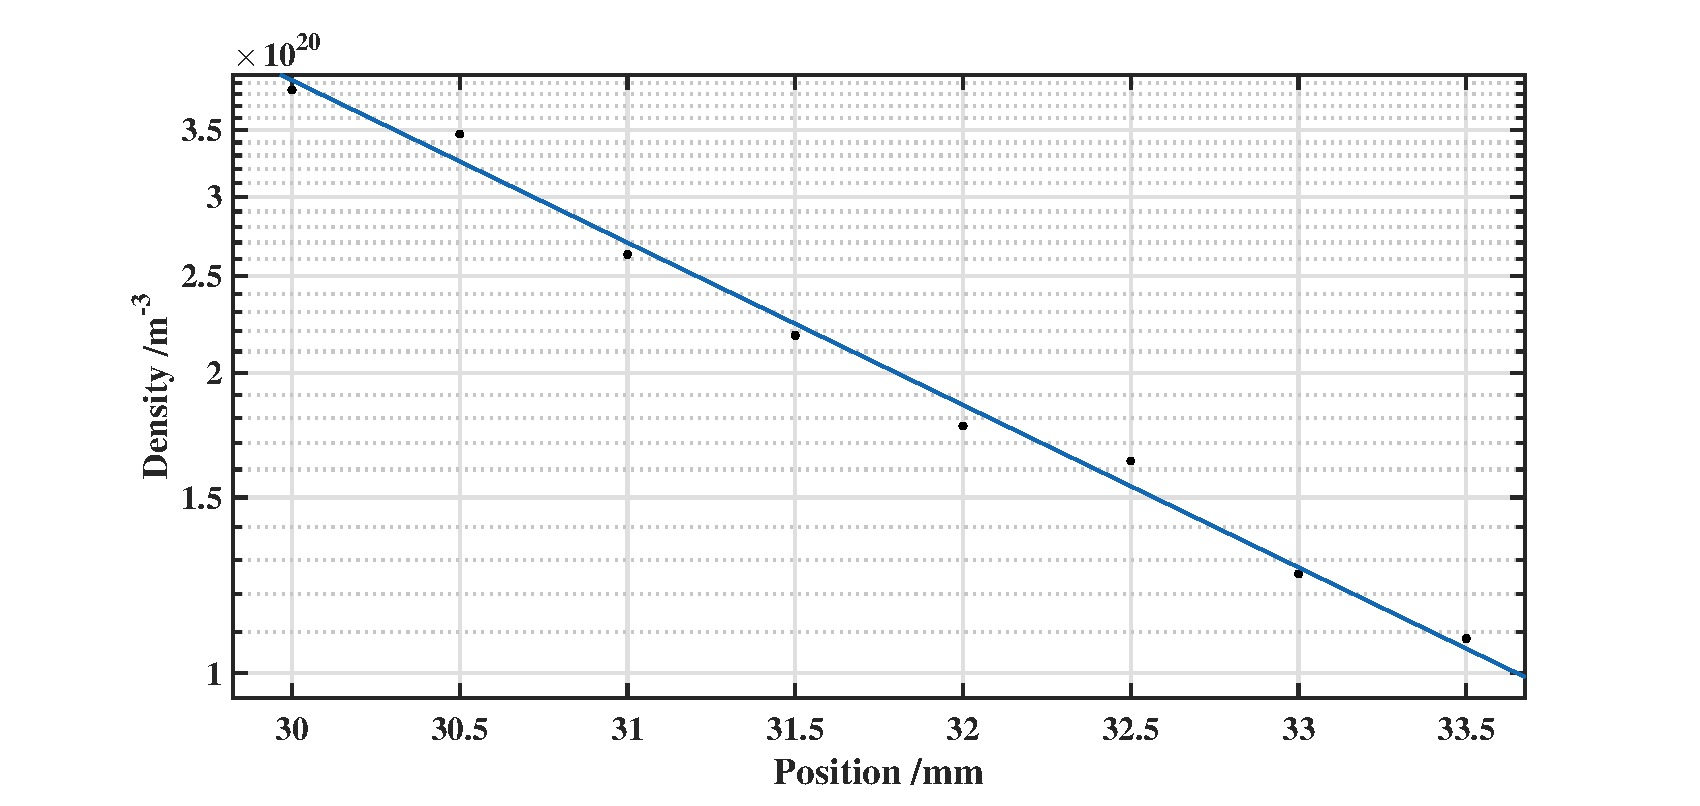
\includegraphics[width=\textwidth]{Figures/OHDecayBig.eps}
	\caption{Figure showing the rapid decay of $\cdot$OH beyond the ends of the plasma channel. The position in the plasma source is shown on the x axis in mm, and the corresponding $\cdot$OH density is shown in m\textsuperscript{-3} on the logarithmic scale y axis. The 30 mm point is the end of the electrodes and 33.5 mm is the last point where the measurement could be taken before the LED was blocked by the casing of the plasma source. The plasma was operated at 10.9 W with a feed gas flow rate of 5slm with 5400 ppm water.}
	\label{fig:OH decay}
\end{figure}

The aim of this experiment was to show how the distance from the gas inlet, and therefore, the position along the 30 mm electrode, affects the density of hydroxyl radicals. Figure \ref{fig:SpatialRes}.
Further to this, it was also possible to assess the densities of $\cdot$OH up to 3.5 mm beyond the end of the electrodes, in order to assess the rate of decay of $\cdot$OH beyond the end of the plasma channel.
This is relevant when considering treatments using plasma jets where the biological sample is likely to be a short distance away from the end of the jet therefore, the species present at this point need to be assessed.
It also is able to provide information on the decay rate of hydroxyl radicals at the end of the electrodes.

To carry out the experiment, the highest power that can be supplied to the setup before causing arcing was used, 10.9W.
In addition to the measurements taken during the experiment, the plasma chemistry was also simulated using a global model developed and run by Sandra Schr\"{o}ter using input plasma parameters to match the experiment.
This is a global model of the plasma which contains over 300 reactions and their rate constants (probabilities that they will happen). It also takes into account the plasma input parameters such as plasma volume, feed gas flow rate and power. In addition, a pathway analysis can be completed to indicate the dominant processes for the production and destruction of individual species.

The data acquired by both experiments (red triangles) and simulation (black dots) are shown in figure \ref{fig:SpatialRes}.
The graph shows that there is a sharp increase from 0-2.5 mm, followed by a smaller increase and decrease to give a little hump seen in both the experimental and simulated data. Following this there is an increase in density over the rest of the channel.
The experimental and simulated data shows excellent agreement.
From figure \ref{fig:PowerVariation}, the accuracy of the experimental densities is expected to be less than $\pm$ 0.5 x 10\textsuperscript{20} m\textsuperscript{-3}, which is greater than the difference between the experimental and simulated densities.

Overall there is the trend of a sharp increase at the start of the plasma channel, followed by a small increase and decrease, the a general increase in density to the end of the channel. 
However, the change in density is very small (less than 1 x 10\textsuperscript{20} m\textsuperscript{-3}), therefore it seems that the position along the plasma channel does not have a massive effect on the $\cdot$OH density.
Using data from the model, the dominant reaction for the formation of $\cdot$OH electron impact causing dissociation of $H_2O$ ($e^- + H_2O \rightarrow H + OH + e^-$), followed by $H + HO_2 \rightarrow OH + OH$.

To interrogate the decrease in $\cdot$OH density beyond the end of the electrodes, measurements were taken every 0.5 mm from the end of the channel to the edge of the window to increase the spatial resolution.
A curve was then fitted to the data points to see the decay of hydroxyl radicals with distance from the end of the electrodes.
As shown in figure \ref{fig:SpatialRes}, there is a rapid, significant decrease in $\cdot$OH density beyond the end of the electrodes.

By plotting the decay on a log scale, as shown in figure \ref{fig:OH decay}, it gives an idea as to how many decay processes are occurring. The linear relationship seen over the full decay would suggest that there is one dominant decay process. 
The information provided by the model suggests that the dominant reactions causing loss of $\cdot$OH are as follows:
\begin{equation}
OH + H_2O_2 \rightarrow  HO_2 + H_2O
\end{equation}
\begin{equation}
OH +HO_2 \rightarrow O_2 +H_2O
\end{equation}
\begin{equation}
OH + OH \rightarrow H_2O_2
\end{equation}

Whilst this shows more than one decay process occurring, at present, the experimental accuracy limits the ability to determine whether there are one or 3 decay processes occurring.
Further measurements and/or species data are required to benchmark the model so that it can be used as an interpretation tool.
In the future, to improve experimental accuracy, it would be of use to be able to make sure the plasma source is definitely fully aligned so that the limits of the electrodes are well defined.

Further to this, it is worth noting that in the model, beyond the 30 mm point, there is no power at all. However, in the experimental setup, the casing of the source is acting as the grounded electrode and therefore continues further than the driven electrode. This could result in coupling between the driving and grounded electrode beyond the 30 mm channel and influence $\cdot$OH.

\section{Discussion}


\subsubsection{Densities of $\cdot$OH}

As mentioned in section \ref{sec:HydroxylRadical}, the concentration of $\cdot$OH required to kill and/inactive cells was 1.9 x 10\textsuperscript{22} m\textsuperscript{-3} (\cite{Attri2015}) and 0.3 $\mu$M (\cite{Zweier1988}).
From the results presented in this report, the maximum density of $\cdot$OH radicals produced was 5 x 10\textsuperscript{20} m\textsuperscript{-3}, which is equivalent to 2.7 x 10 \textsuperscript{-4} $\mu$M.
This shows that the densities of $\cdot$OH in the plasma described in this report are several orders of magnitude lower than that required to kill cells.
This suggests that to be biologically relevant, the density of $\cdot$OH produced in the plasma must be increased.

Further to this, the densities obtained from the data presented here is from within the plasma channel, an area that cannot be directly applied to a target.
This means that actually, the densities of the effluent are the important part, as the target sample during a plasma treatment in likely to be in the order of a few cm from the end of the plasma jet.


\subsubsection{Spatial Resolution and $\cdot$OH decay}
From the spatial resolution data in \ref{subsec:SpatialRes}, the lifetime of $\cdot$OH was shown to be very short and that the densities decreased very rapidly, almost to nothing, in only 3.5 mm after leaving the plasma channel. 
The decay process shown in \ref{subsec:SpatialRes} shows that the lifetime of $\cdot$OH is very short and therefore, almost all $\cdot$OH is lost early in the effluent. 
This raises a problem with using $\cdot$OH as a therapy as it is so short lived it is likely to never meet it's biological target.
There are two obvious ways of approaching this problem. Firstly, raising the $\cdot$OH density in the plasma channel so it lasts longer beyond the channel, and secondly, instead of looking at the direct effect of plasma-produced $\cdot$OH, look at the biological action of it's secondaries and how they are affected by $\cdot$OH density

\subsubsection{Raising $\cdot$OH density}

One way to increase the $\cdot$OH density in the plasma and effluent would be to increase the power in the system which should result in a higher electron density, increased electron energy and therefore increased dissociation.
Unfortunately, this is not possible with the setup used as plasma powers greater than 10.9W caused arcing.
However, in the future, it would be worth increasing the frequency of the driving electrode as this should have a similar effect as increasing the power (i.e. increasing the density of $\cdot$OH), without causing arcing of the plasma.

Results also showed that increasing the water content of the feed gas increased the $\cdot$OH density, though the percentage dissociation decreased with increasing water. 
The increased frequency may also be able to increase the dissociation of water, thus allowing greater densities of $\cdot$OH to be achieved.
 

\subsubsection{Products of $\cdot$OH Consumption}

The dominant reactions for $\cdot$OH consumption in the effluent, according to the global model, are $ OH + H_2O_2 \rightarrow HO_2 + H_2O$, $OH + HO_2 \rightarrow O_2 + H_2O$ and $OH + OH \rightarrow H_2O_2$.
It is therefore of interest to understand the actions of these secondary products in biological environments, and how manipulation of $\cdot$OH density affects their production. 
Hydroperoxyl radical ($HO_2$) is able to react with fatty acids and $H_2O_2$ is able to easily cross cell membranes and cause damage from producing $\cdot$OH in the presence of transition metals \cite{Phaniendra2015}.
It may be that by altering $\cdot$OH production in plasma, it is indirectly causing damage to cells through production of these secondaries.

Another factor of importance when considering the decay of $\cdot$OH in terms of plasma treatment, is the different interfaces that the effluent will come into contact with \cite{Hirst2016}.
Firstly, the air between the jet and the sample will contain different gases and molecules which may affect the lifetime and activity of the plasma-produced RONS.
Secondly, the surface for treatment, such as a skin lesion, will have fluid on it as a result of the inflammatory process occurring there.
This fluid will contain proteins and other components which may also affect the lifetime and reactivity of RONS.
It is therefore important to consider these things when developing successful therapies as they will effect the nature of the plasma species that need to be produced in the plasma initially.

\subsubsection{Alterations to the Plasma Setup}

During the measurements to determine the spatial resolution of $\cdot$OH, the plasma source was mounted on a stage which could be moved horizontally and vertically by fractions of a mm.
However, the stage and source was not totally solid so when moving the source up and down to take the different measurements, there may have been some twisting/leaning. This meant that repeated fine adjustment of the source was required to maintain a strong LED signal. 
This in turn may mean that the error in the actual position where the measurement was taken may be increased. 

Further to this alignment issue, it is hard to find the ends of the electrodes accurately and therefore hard to define the exact ends of the plasma channel when using the setup as it is.
This is something that would be good to improve therefore it would be worth investigating whether there is a method for accurately determining where the ends of the electrodes are in order to improve the accuracy of the positions where measurements were taken.

Another adaptation to the setup that would prove useful in further interrogating the plasma effluent would be to increase the length of the effluent region (ie, longer than 3.5 mm), so that plasma diagnostics such as absorption spectroscopy could be carried out over a greater range of this region.
This would give more of an insight into the plasma components that may be capable of reaching biological targets a matter of cm away from the end of the jet.


\subsubsection{Outlook}

By understanding the underlying mechanisms of RONS production in plasma, and their interactions with biological samples, it may be possible to produce finely tuned plasmas which are capable of producing well-characterised effluents for a range of therapeutic uses.
Meanwhile, it would be of use to be able to characterise the effects of individual RONS on various different types of bacteria, commonly present in wounds, in order to understand what the optimal plasma treatment would be.

Further to this, it would be interesting to understand whether or not combined therapy could prove useful in the treatment of infected wounds. 
For example, would administration of antibiotics alongside plasma treatment prove more effective than either therapy alone?
This would be an interesting question to investigate as it may be that antibiotics could potentially be incorporated into plasmas, either intact so that it can act as the plasma effluent reaches the target, or in a pro-drug form that could be catalysed to the active drug in the plasma region itself.
This combined therapy may result in superior therapeutic action as the antibiotics may be able to weaken the bacterial cells, making them more susceptible to plasma treatment.

However, amongst all these positive potential applications for plasma treatments, it is also of utmost importance that the safety of plasma treatment is fully understood. 
Plasma components that could potentially cause harm include plasma temperature and resultant of the target, UV radiation and production of toxic gases and RONS \cite{Weltmann2009}.
Guidelines for these parameters deemed to be safe for patient application exist and therefore the characterisation of plasma jets and the determination of the plasma doses must take these into consideration.

In conclusion, the production of RONS by low temperature plasmas could provide an interesting alternative therapy for the treatment of different conditions, such as wound infections. This could prove particularly exciting at this time of rising antibiotic resistance.

%Dose-response curves?
%Treatment and rests like chemotherapy

\bibliographystyle{unsrt}
\bibliography{MyPapers}

\end{document}  